\subsubsection{LOG} \label{subsubsec:log}

Las Figs. \ref{fig:Hval_Log} a \ref{fig:MP_Log} muestran las propiedades estadísticas del mapa LOG en representación de coma flotante y punto fijo.
Todas estas figuras muestran: $100$ puntos rojos (surrogados) por cada precisión de punto fijo ($1 \geq B \geq 53$) y en negro su promedio (línea negra discontinua que conecta puntos negros), $100$ líneas discontinuas horizontales azules que son el resultado de cada surrogado en punto flotante y una línea continua negra en su promedio.
Tenga en cuenta que estas líneas son independientes del eje x.
En este caso, todas las líneas del punto flotante se superponen.

Según $B$ crece, las propiedades estadísticas varían hasta que se estabilizan.
Para $B \geq 30$, el valor de $H_{hist}$ permanece casi idéntico al valor de la representación en coma flotante, mientras que $H_{BP}$ y $C_{BP}$ se estabilizan a $B > 21$.
Sus valores son: $\left\langle H_{hist}\right\rangle = 0.9669$; $\left\langle H_{BP}\right\rangle = 0.6269$; $\left\langle C_{BP}\right\rangle = 0.4843$.
Tenga en cuenta que el valor estable de los patrones faltantes $MP = 645$ hace que el valor óptimo sea $H_{BP} \leq \ln(75)/\ln(720) \simeq 0.65$.
Entonces, $B = 30$ es la opción más conveniente para la implementación en hardware porque un aumento en el número de dígitos fraccionarios no mejora las propiedades estadísticas.

Se pueden sacar algunas conclusiones con comparando los cuantificadores de BP y BPW.
Para $B = 1, 2, 3$ y $4$, los cuantificadores de BP promediados son casi $0$ mientras que los cuantificadores de BPW promediados no se pueden calcular (ver en las figuras \ref{fig:Hbpw_Log} y \ref{fig:Cbpw_Log} la línea punteada negra faltante).
Esto se debe a que para esas secuencias la condición inicial era $0$, todas las iteraciones resultan ser una secuencia de ceros (el punto fijo del mapa), esto es más probable que ocurra cuando se usan pequeñas precisiones debido al redondeo.

Cuando $B$ aumenta las condiciones iniciales se redondean a cero con menos frecuencia, esto se puede ver para $B > 6$.
En este caso, las secuencias generadas que comienzan desde un valor no nulo caen a cero después de un transitorio cortomuy frecuentemente.
Un tema interesante en las Figs. \ref{fig:Hbpw_Log} y \ref{fig:Cbpw_Log}, es que los cuantificadores de BPW muestran una alta dispersión a diferencia de los cuantificadores de BP.
Esto se debe a que el procedimiento BPW tiene en cuenta transitorios y descarta los puntos fijos, a diferencia del procedimiento BP, que considera todos los valores de la secuencia.
Podemos ver en las Figs. \ref{fig:Hbpw_Log} y \ref{fig:Cbpw_Log} para $1 < B < 10$ líneas horizontales de puntos rojos que no aparecen en las Figs. \ref{fig:Hbp_Log} y \ref{fig:Cbp_Log}, esto evidencia que las diferentes condiciones iniciales caen en las mismas órbitas, incluso para las precisiones adyacentes.
%
\begin{figure}[htpb]
	\centering
	\begin{subfigure}[b]{0.49\textwidth}
		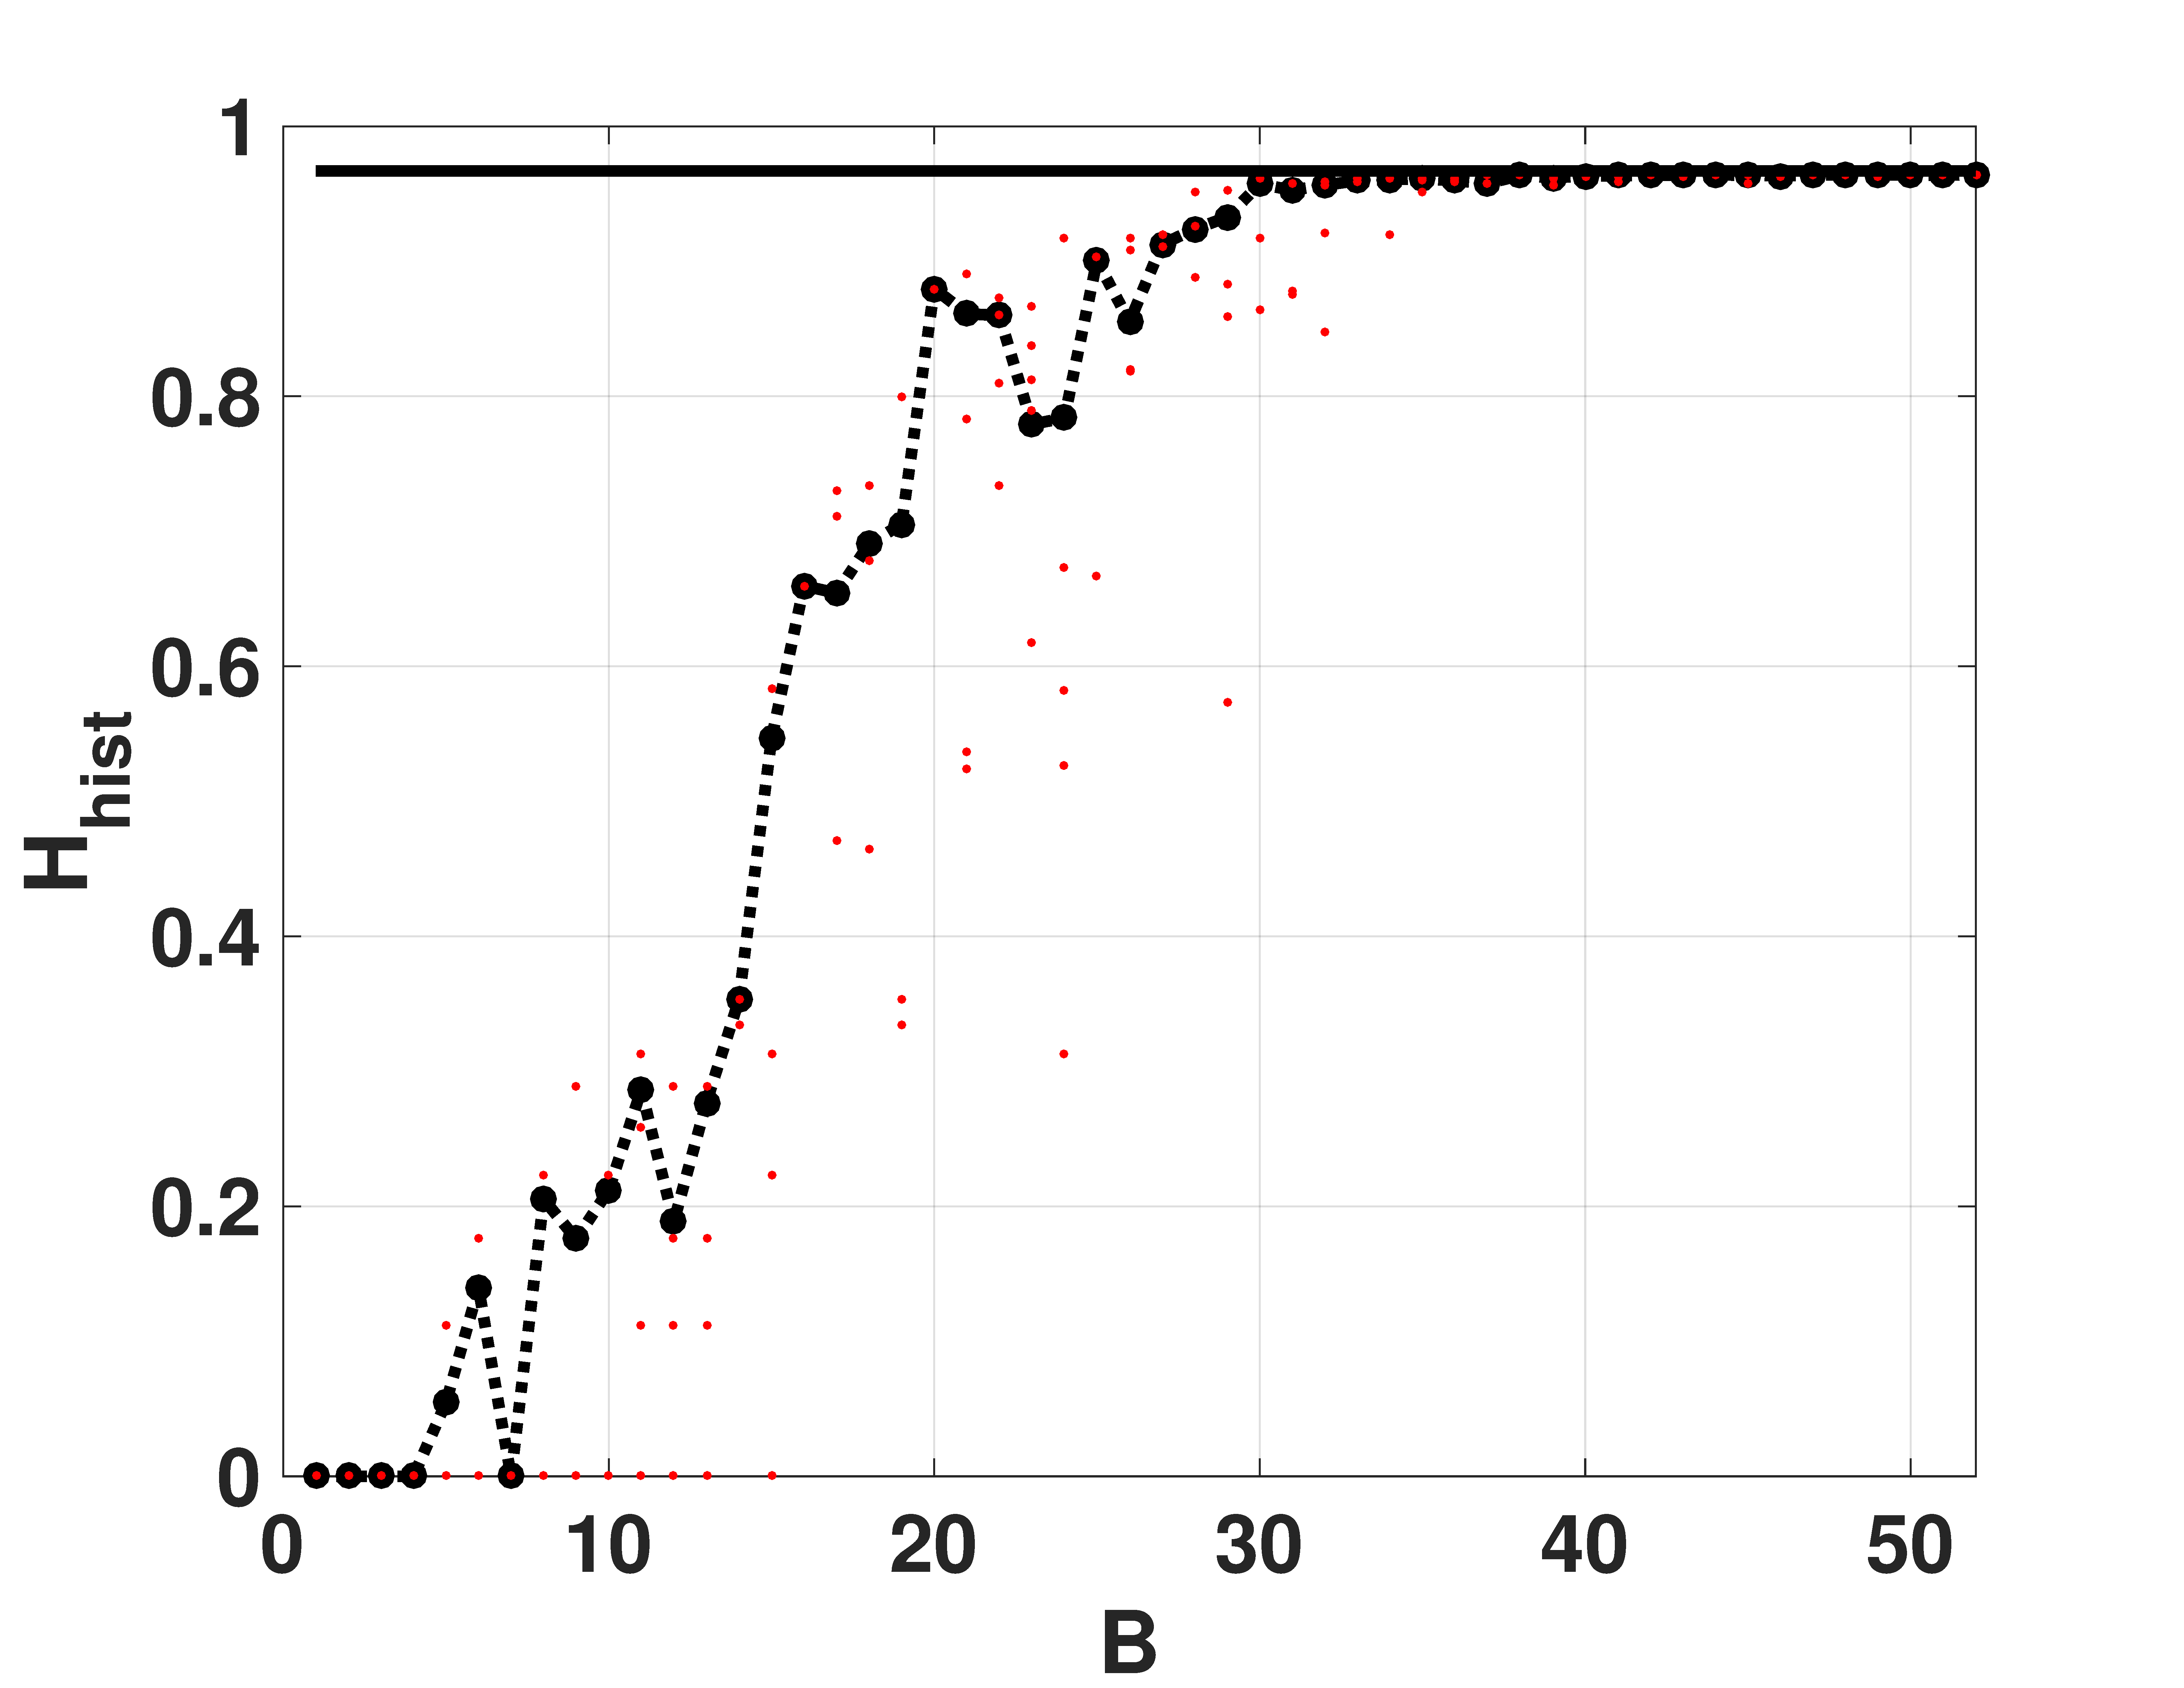
\includegraphics[width=\textwidth]{Hval_Log}
		\caption{$H_{hist}$ vs. $B$}
		\label{fig:Hval_Log}
	\end{subfigure}
	\begin{subfigure}[b]{0.49\textwidth}
		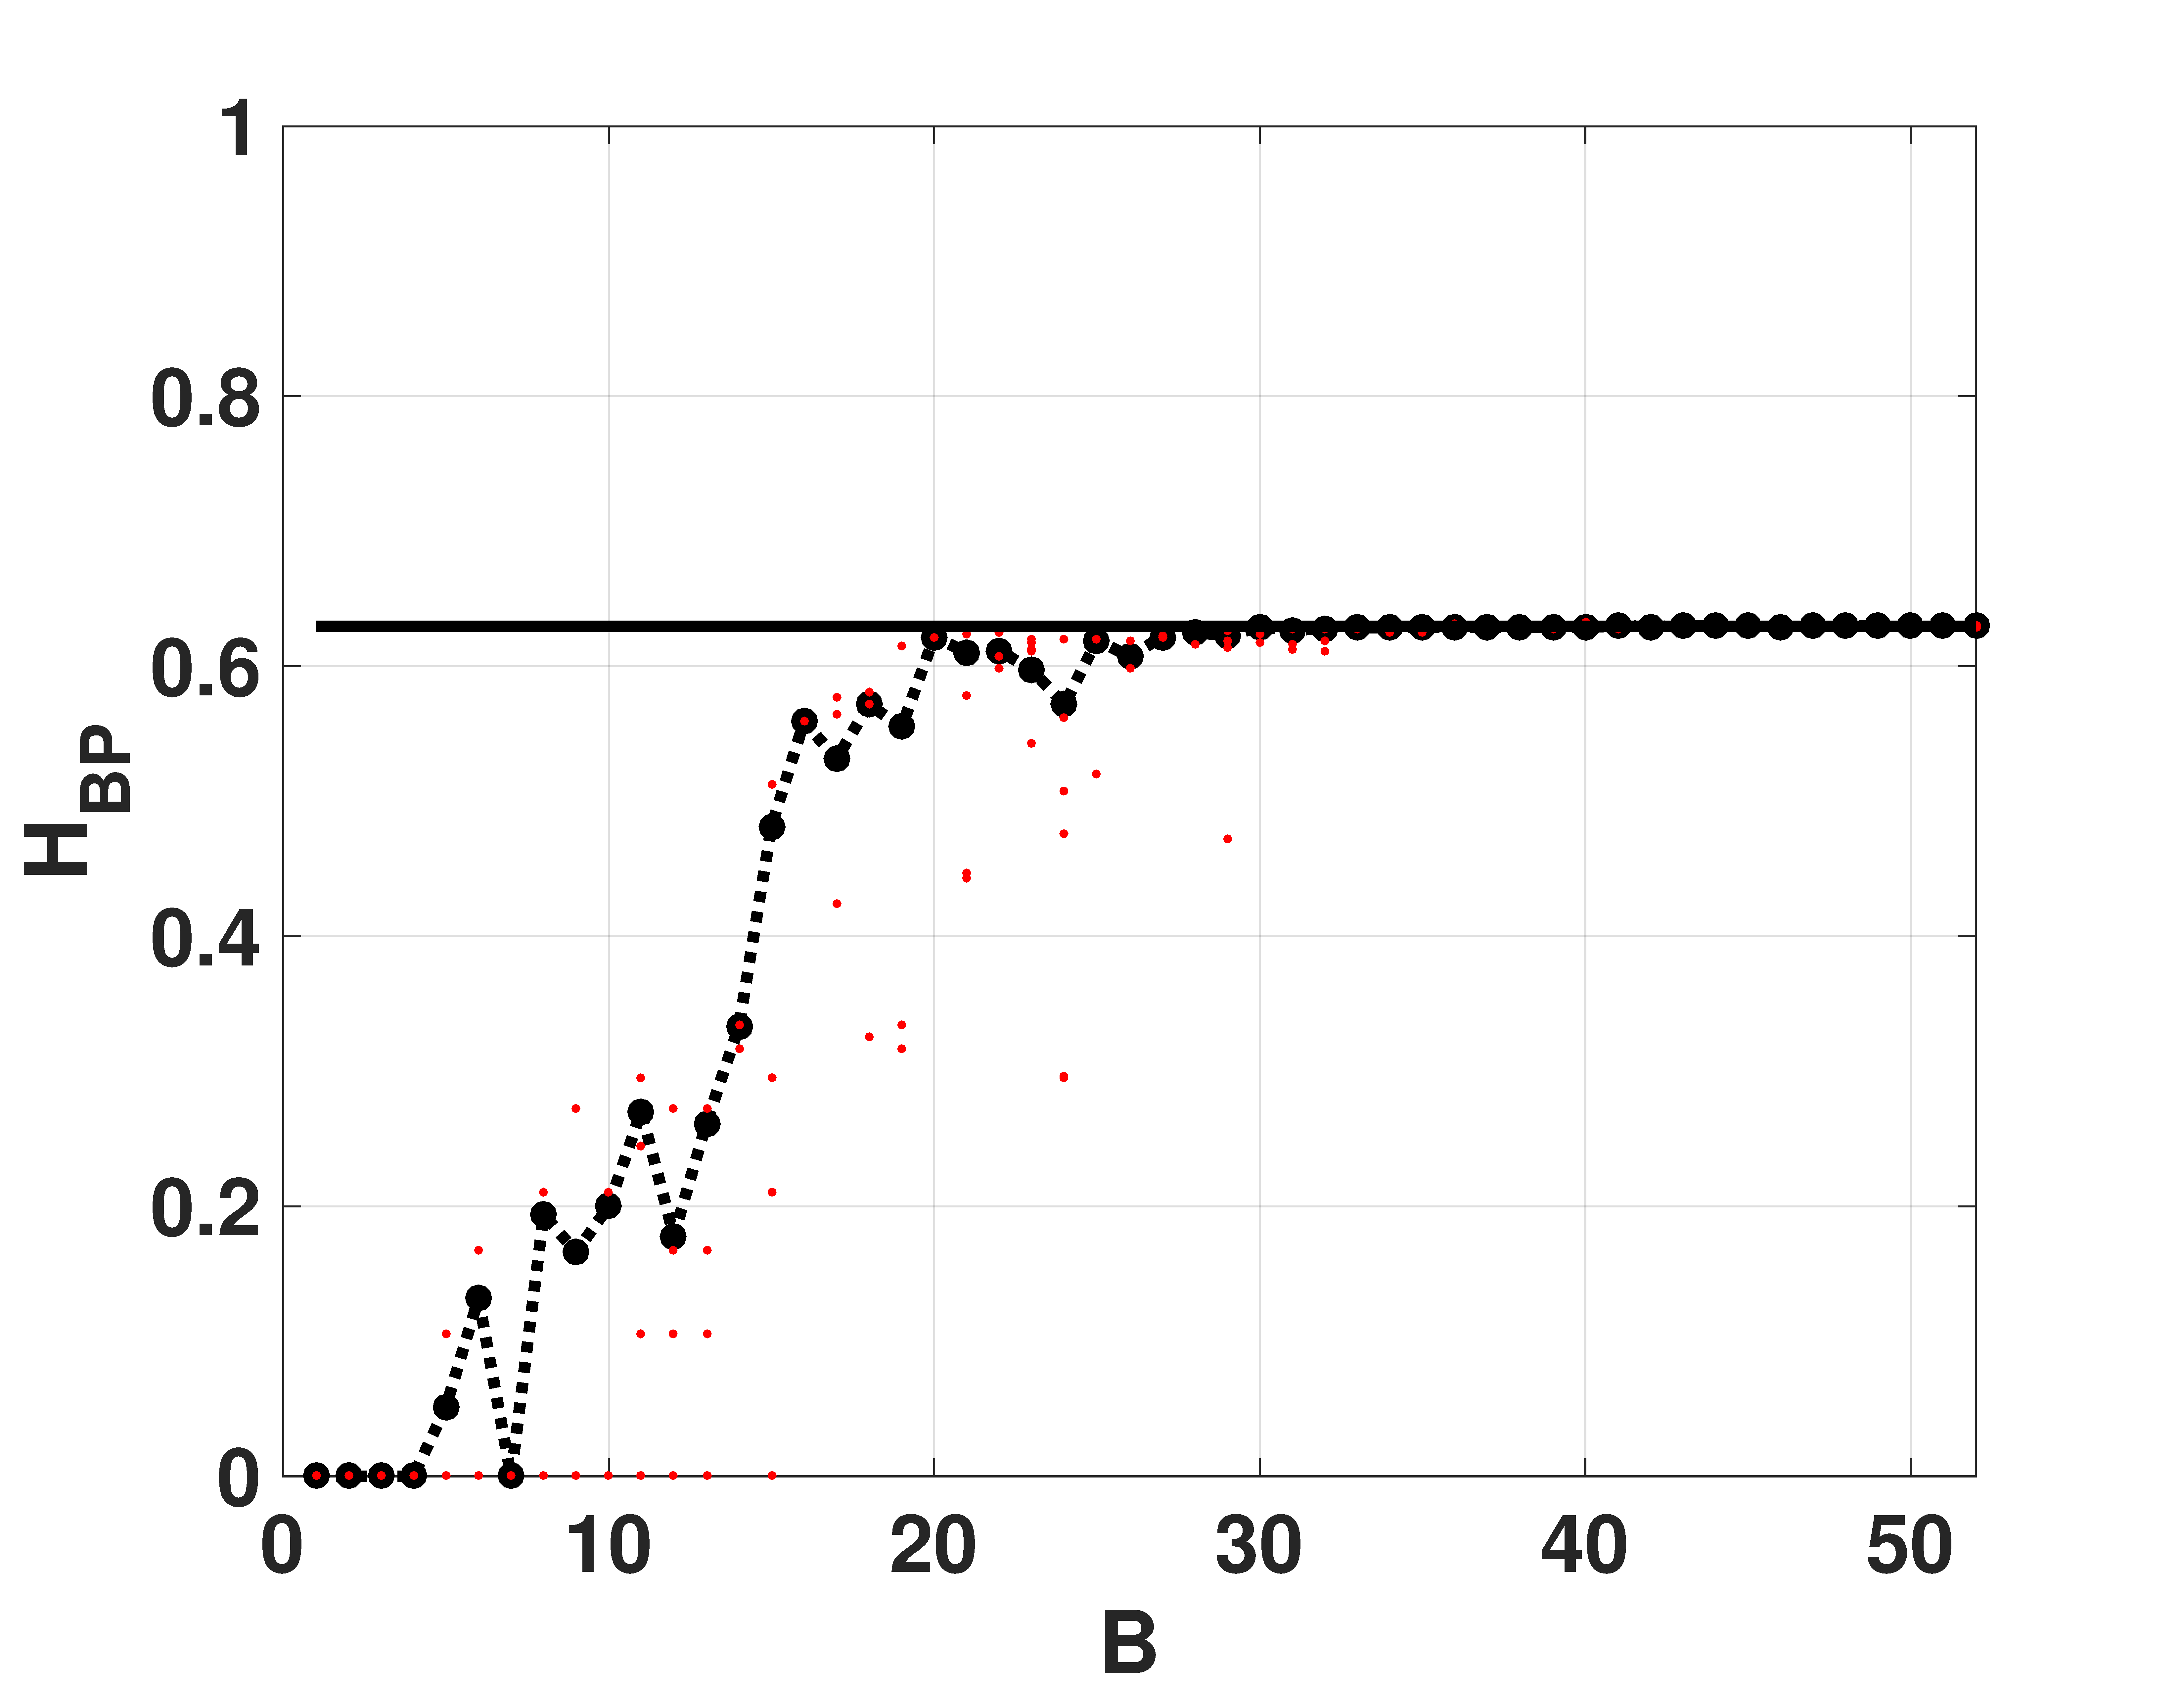
\includegraphics[width=\textwidth]{Hbp_Log}
		\caption{$H_{BP}$ vs. $B$}
		\label{fig:Hbp_Log}
	\end{subfigure}
	\begin{subfigure}[b]{0.49\textwidth}
		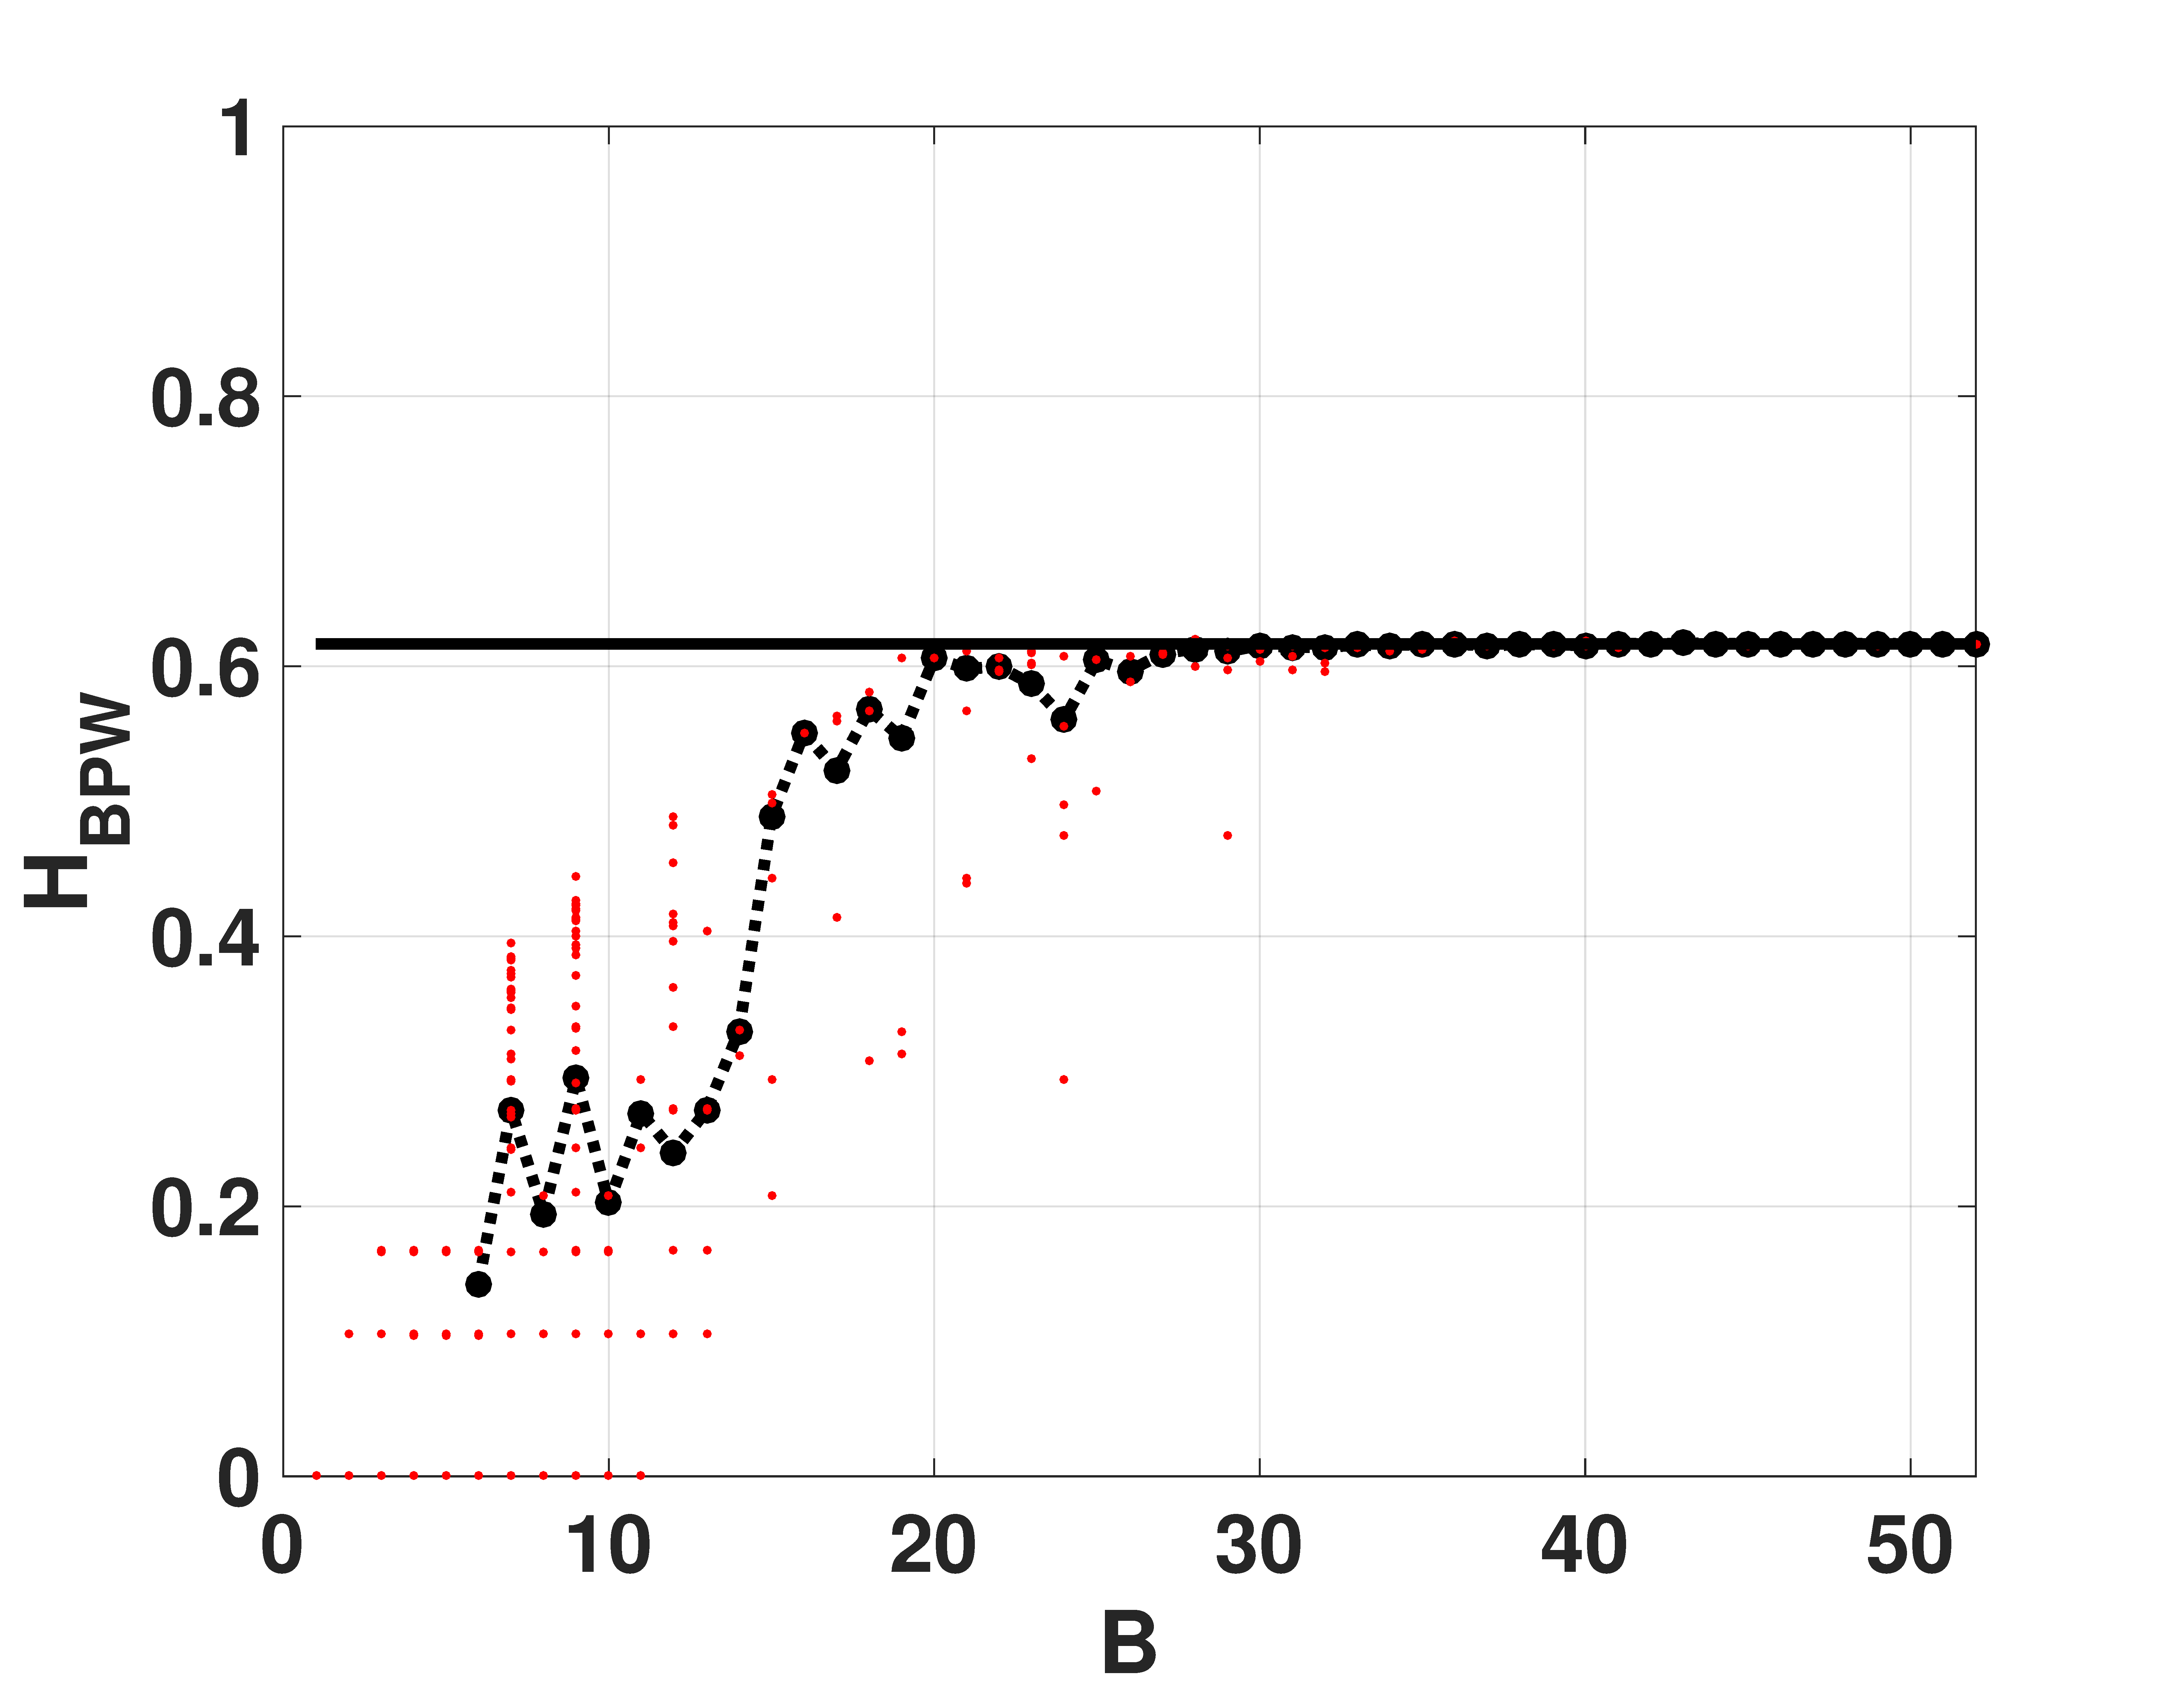
\includegraphics[width=\textwidth]{Hbpw_Log}
		\caption{$H_{BPW}$ vs. $B$}
		\label{fig:Hbpw_Log}
	\end{subfigure}
	\begin{subfigure}[b]{0.49\textwidth}
		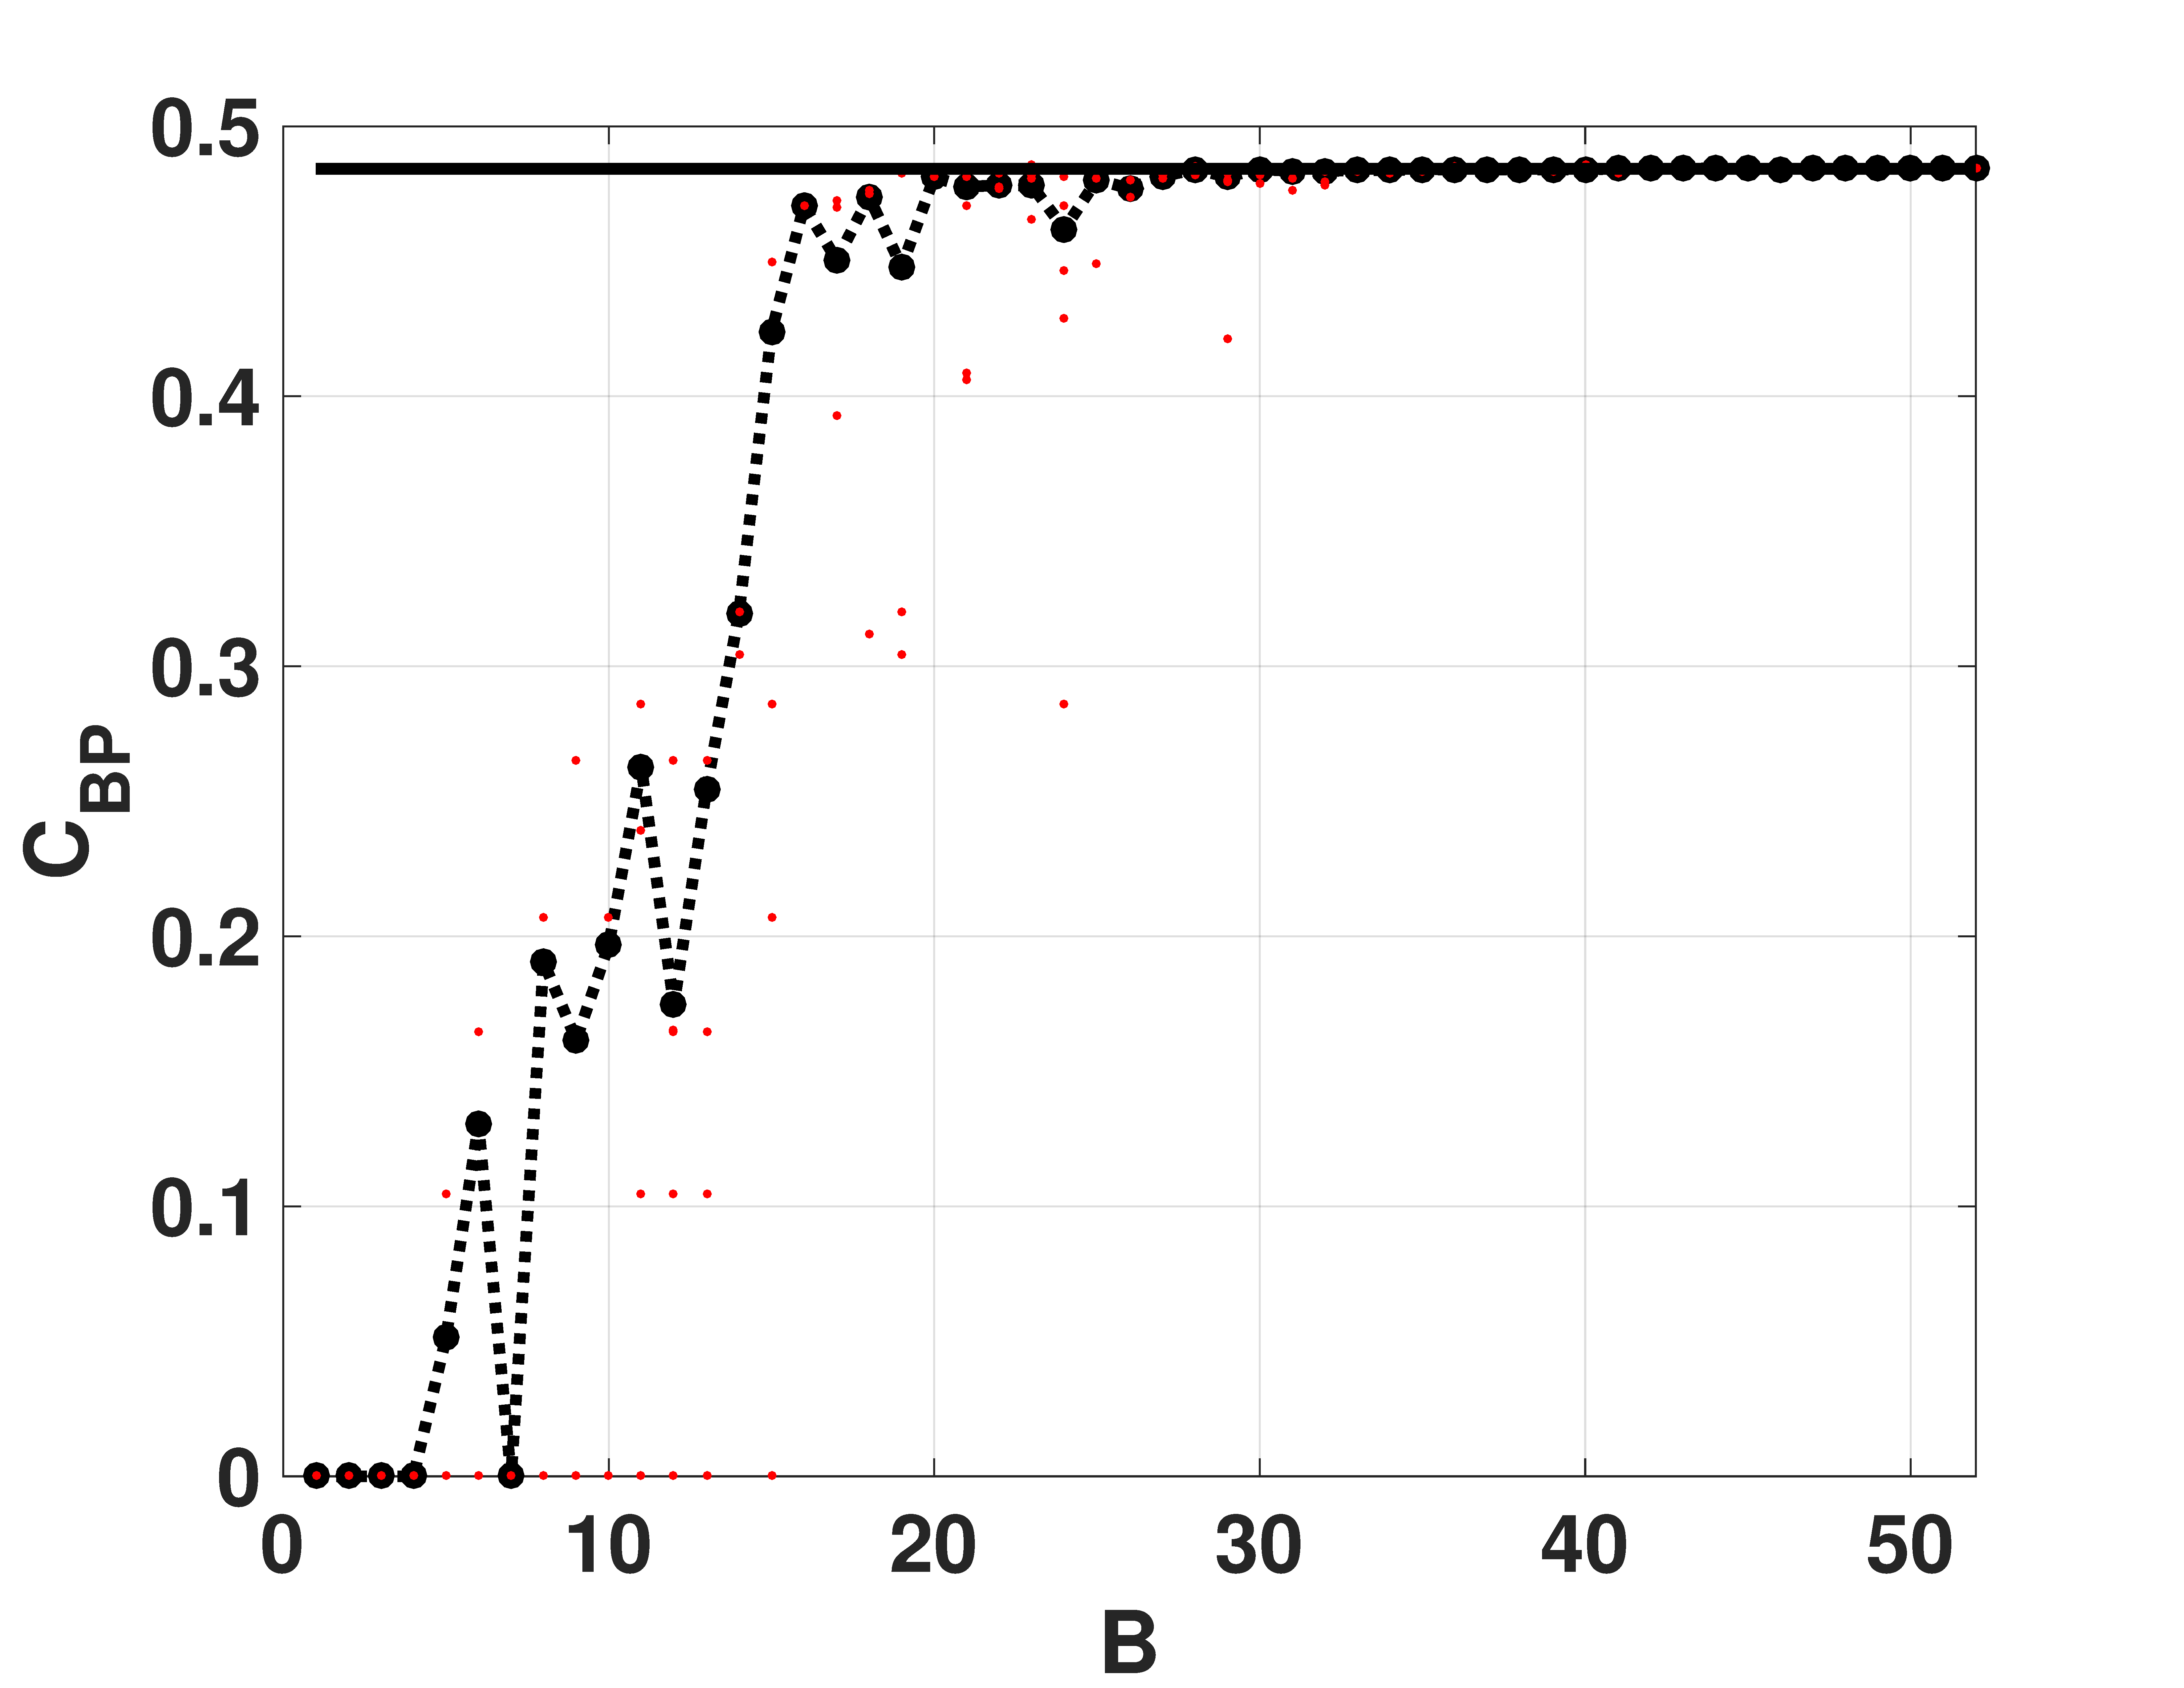
\includegraphics[width=\textwidth]{Cbp_Log}
		\caption{$C_{BP}$ vs. $B$}
		\label{fig:Cbp_Log}
	\end{subfigure}
	\begin{subfigure}[b]{0.49\textwidth}
		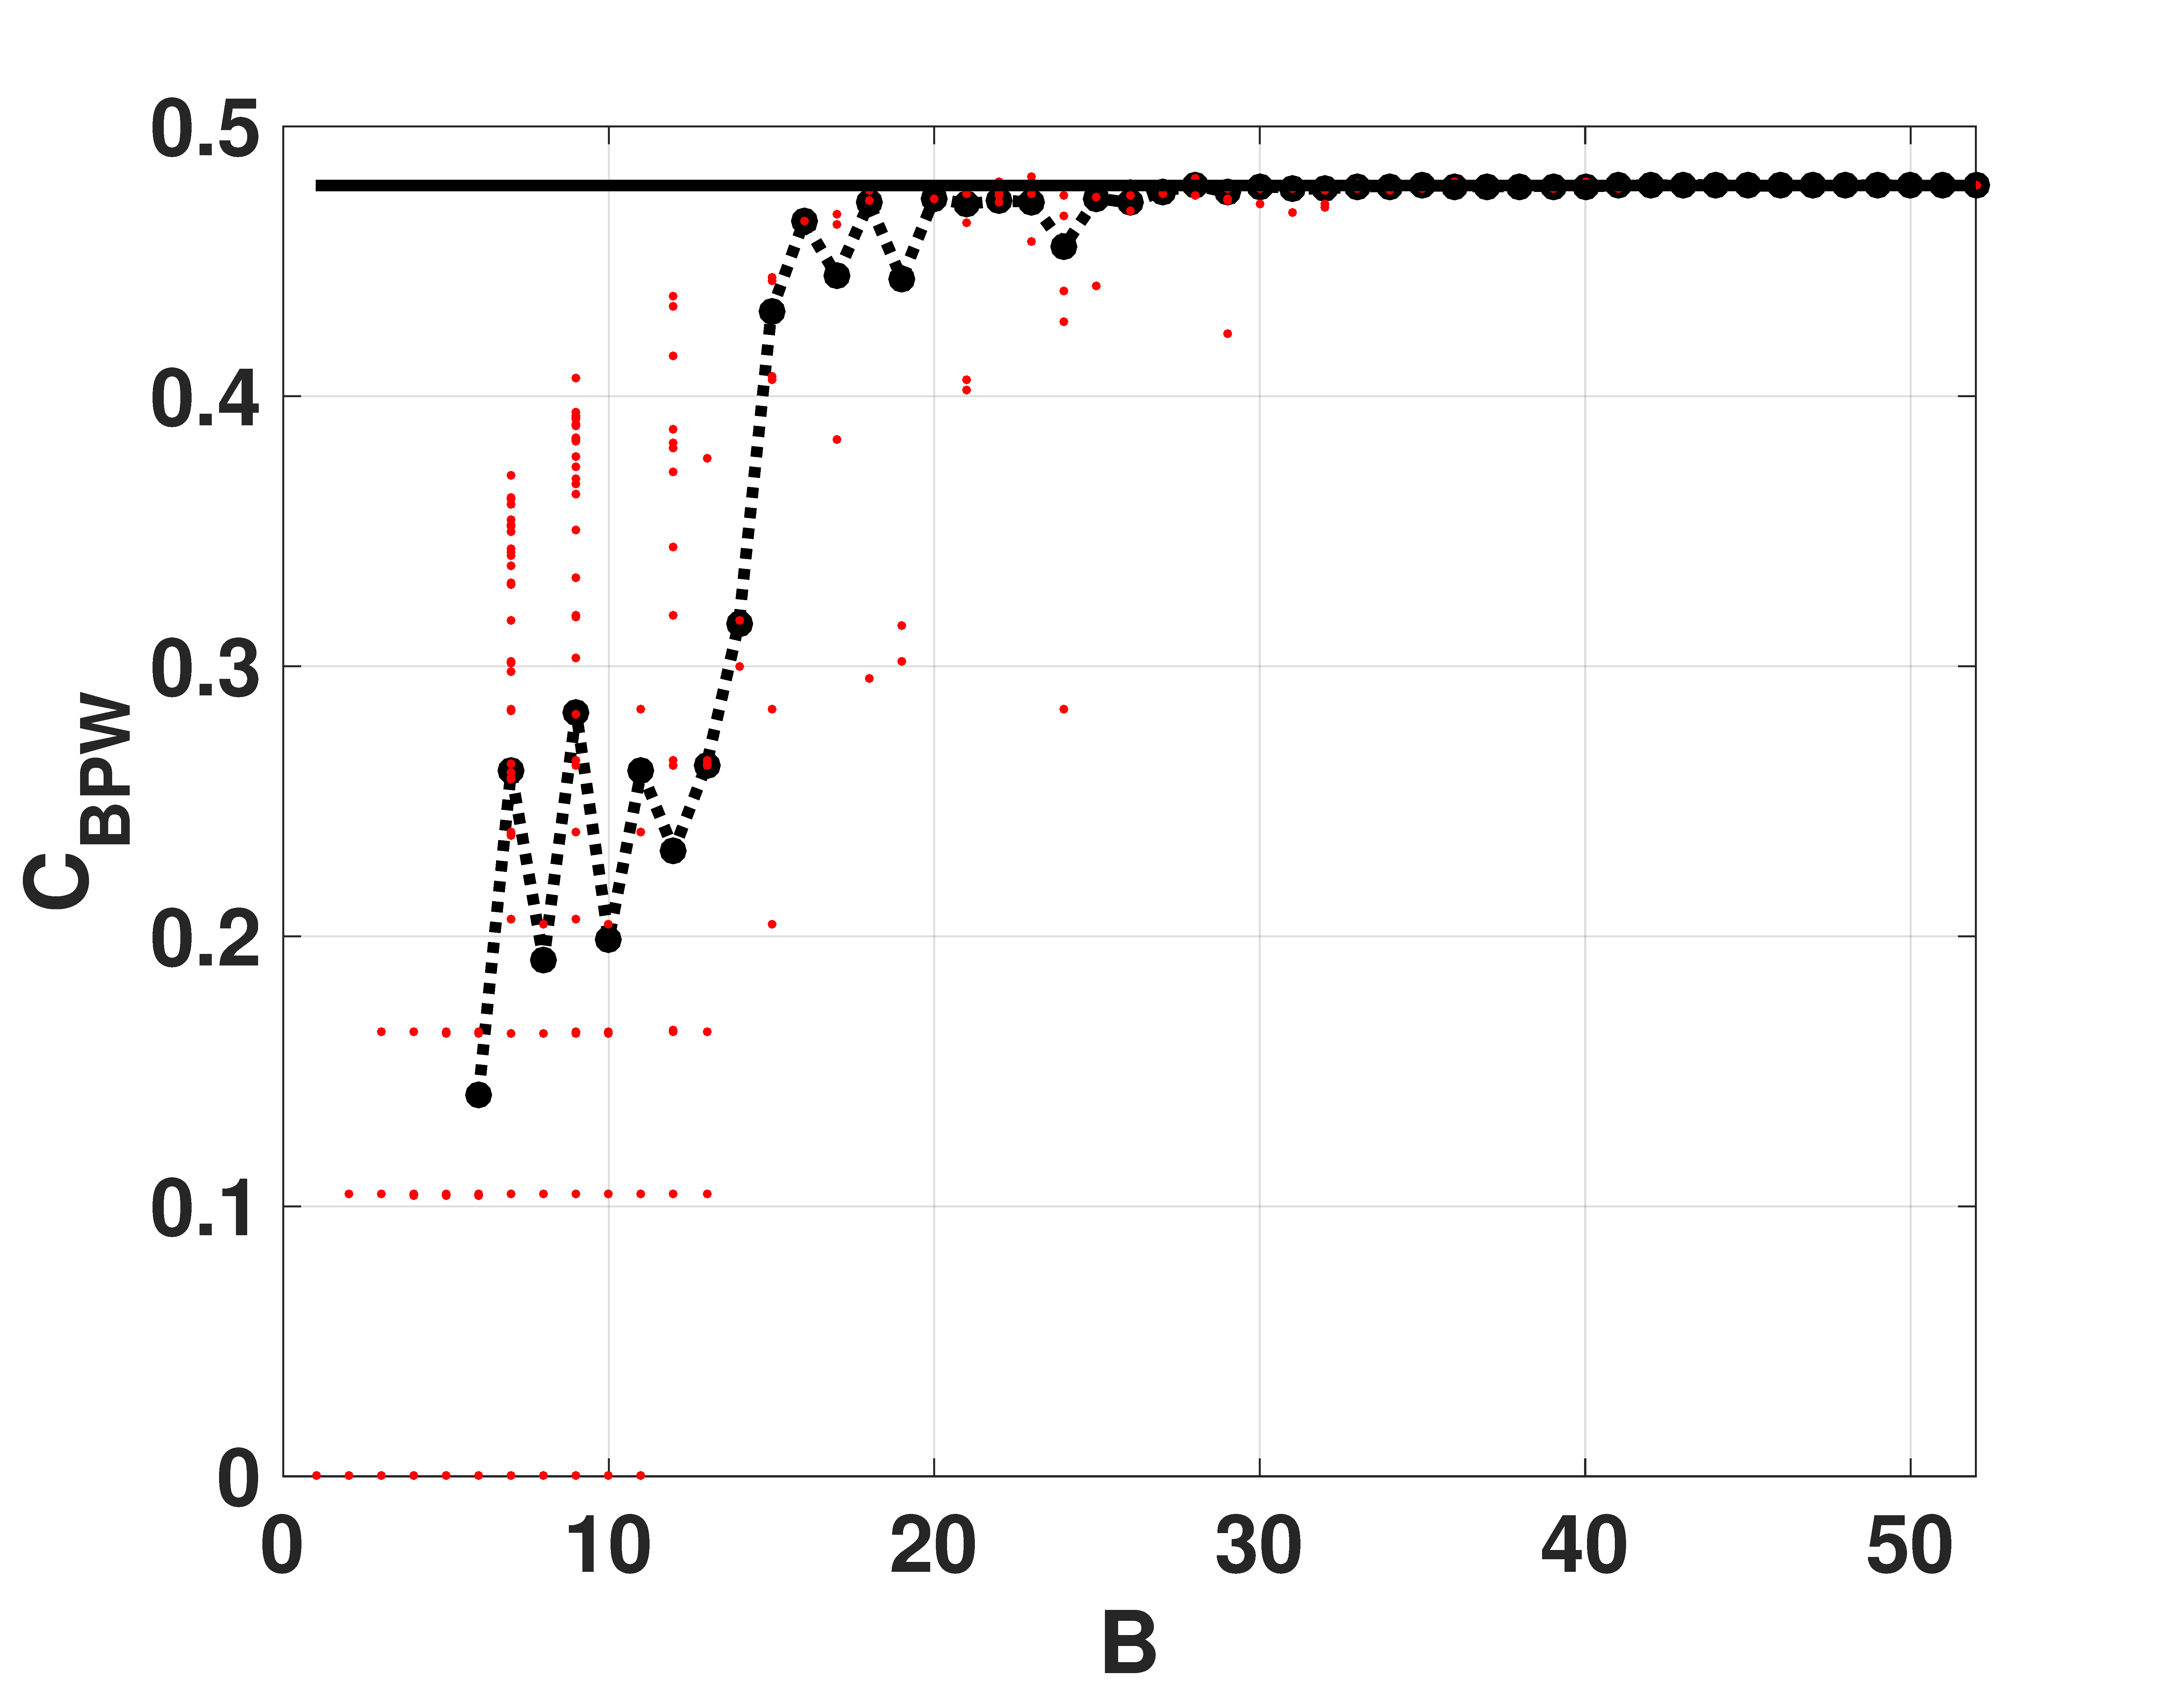
\includegraphics[width=\textwidth]{Cbpw_Log}
		\caption{$C_{BPW}$ vs. $B$}
		\label{fig:Cbpw_Log}
	\end{subfigure}
	\begin{subfigure}[b]{0.49\textwidth}
		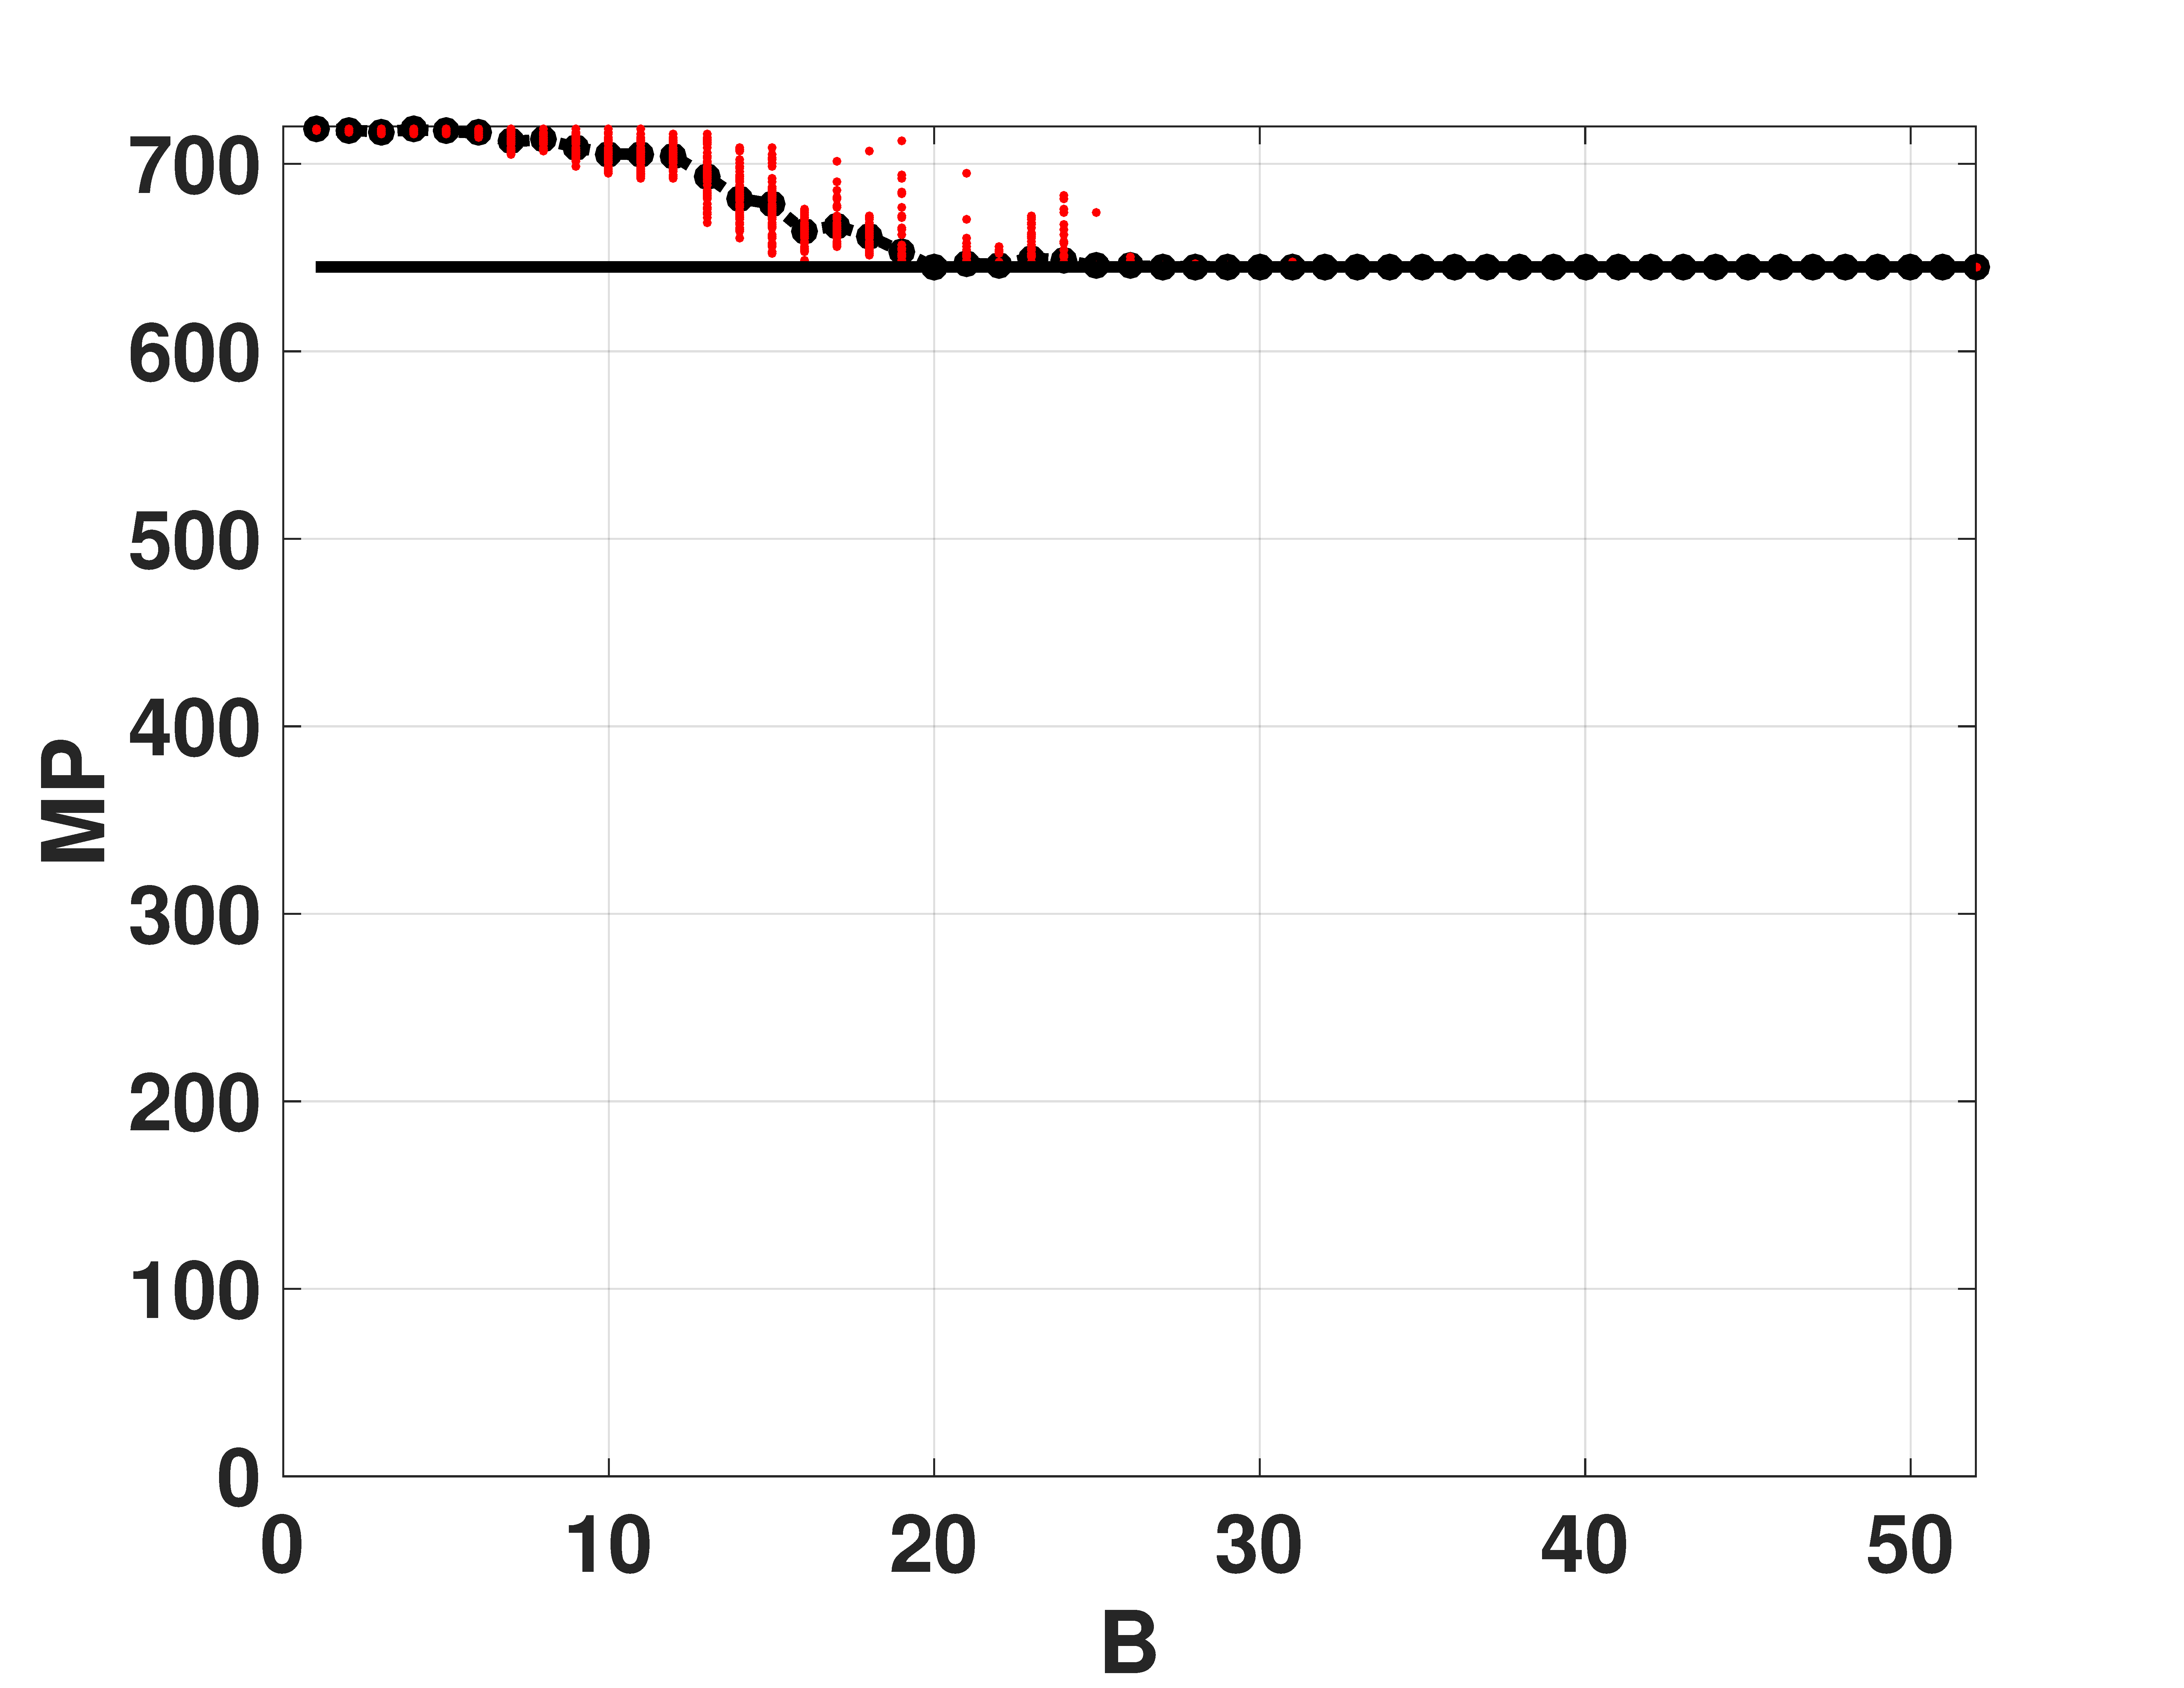
\includegraphics[width=\textwidth]{MP_Log}
		\caption{MP vs. $B$}
		\label{fig:MP_Log}
	\end{subfigure}
	\caption{Propiedades estadísticas para el mapa LOG en función de $B$.}
	\label{fig:LOG_QuantiB}
\end{figure}

Los mismos resultados se muestran en planos de doble entropía con la precisión como parámetro (Fig. \ref{fig:HbpHval_Log} sin contribuciones de amplitud y Fig. \ref{fig: HbpwHval_Log} con contribuciones de amplitud).
Estas figuras muestran: $100$ puntos rojos por cada precisión de punto fijo ($B$) y su promedio en negro (línea negra discontinua que conecta puntos negros), $100$ puntos azules que son los resultados de cada surrogado en coma flotante y la estrella negra es su promedio.
Aquí, los $100$ puntos azules y su promedio se superponen.

Como se esperaba, la implementación de la arquitectura de punto fijo converge al valor de coma flotante a medida que aumenta $B$.
Para ambos planos, $H_{hist} \times H_{BP}$ y $H_{hist} \times H_{BPW}$, desde $B = 20$, $H_{hist}$ aumenta pero $H_{BP}$ y $H_{BPW}$ permanecen constantes.
Se puede ver que la entropía de distribución de valores es alta ($\left \langle H_{hist} \right \rangle = 0.9669$) pero su mezcla es pobre ($\left \langle H_{BP} \right \rangle = 0.6269$).
%
\begin{figure}[htpb]
	\centering
	\begin{subfigure}[b]{0.49\textwidth}
		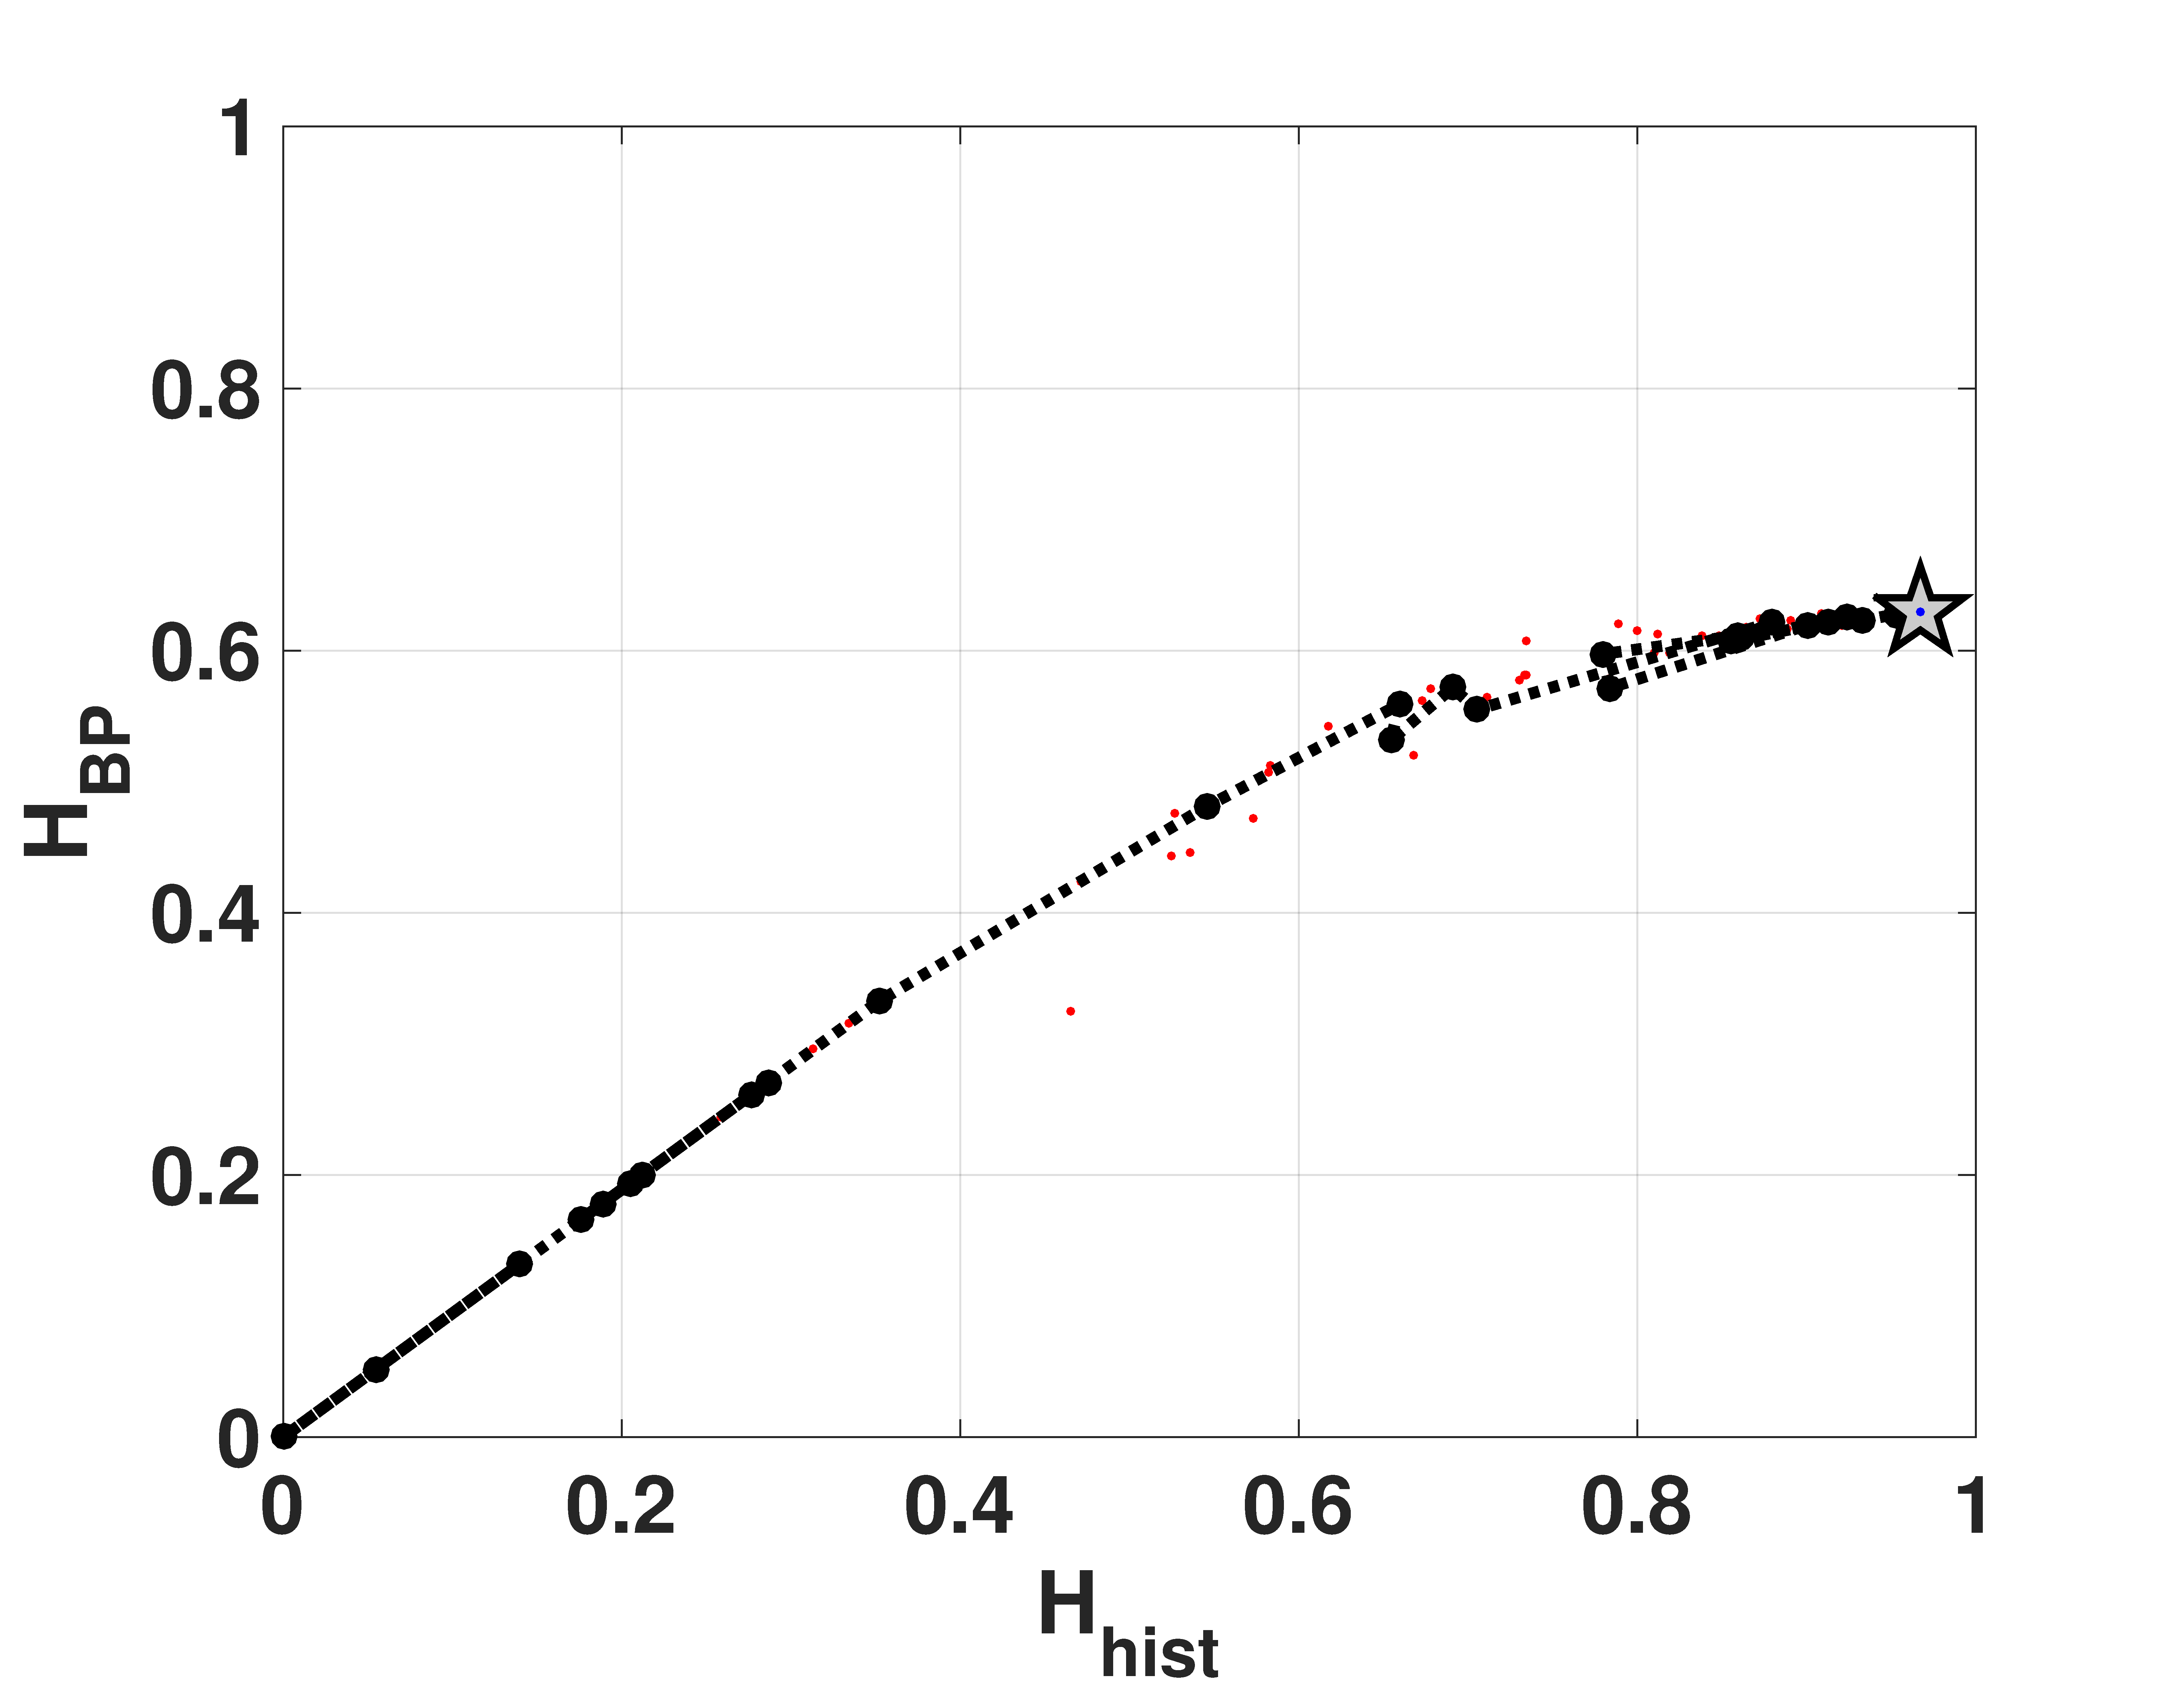
\includegraphics[width=\textwidth]{HbpHval_Log}
		\caption{$H_{hist} \times H_{BP}$}
		\label{fig:HbpHval_Log}
	\end{subfigure}
	\begin{subfigure}[b]{0.49\textwidth}
		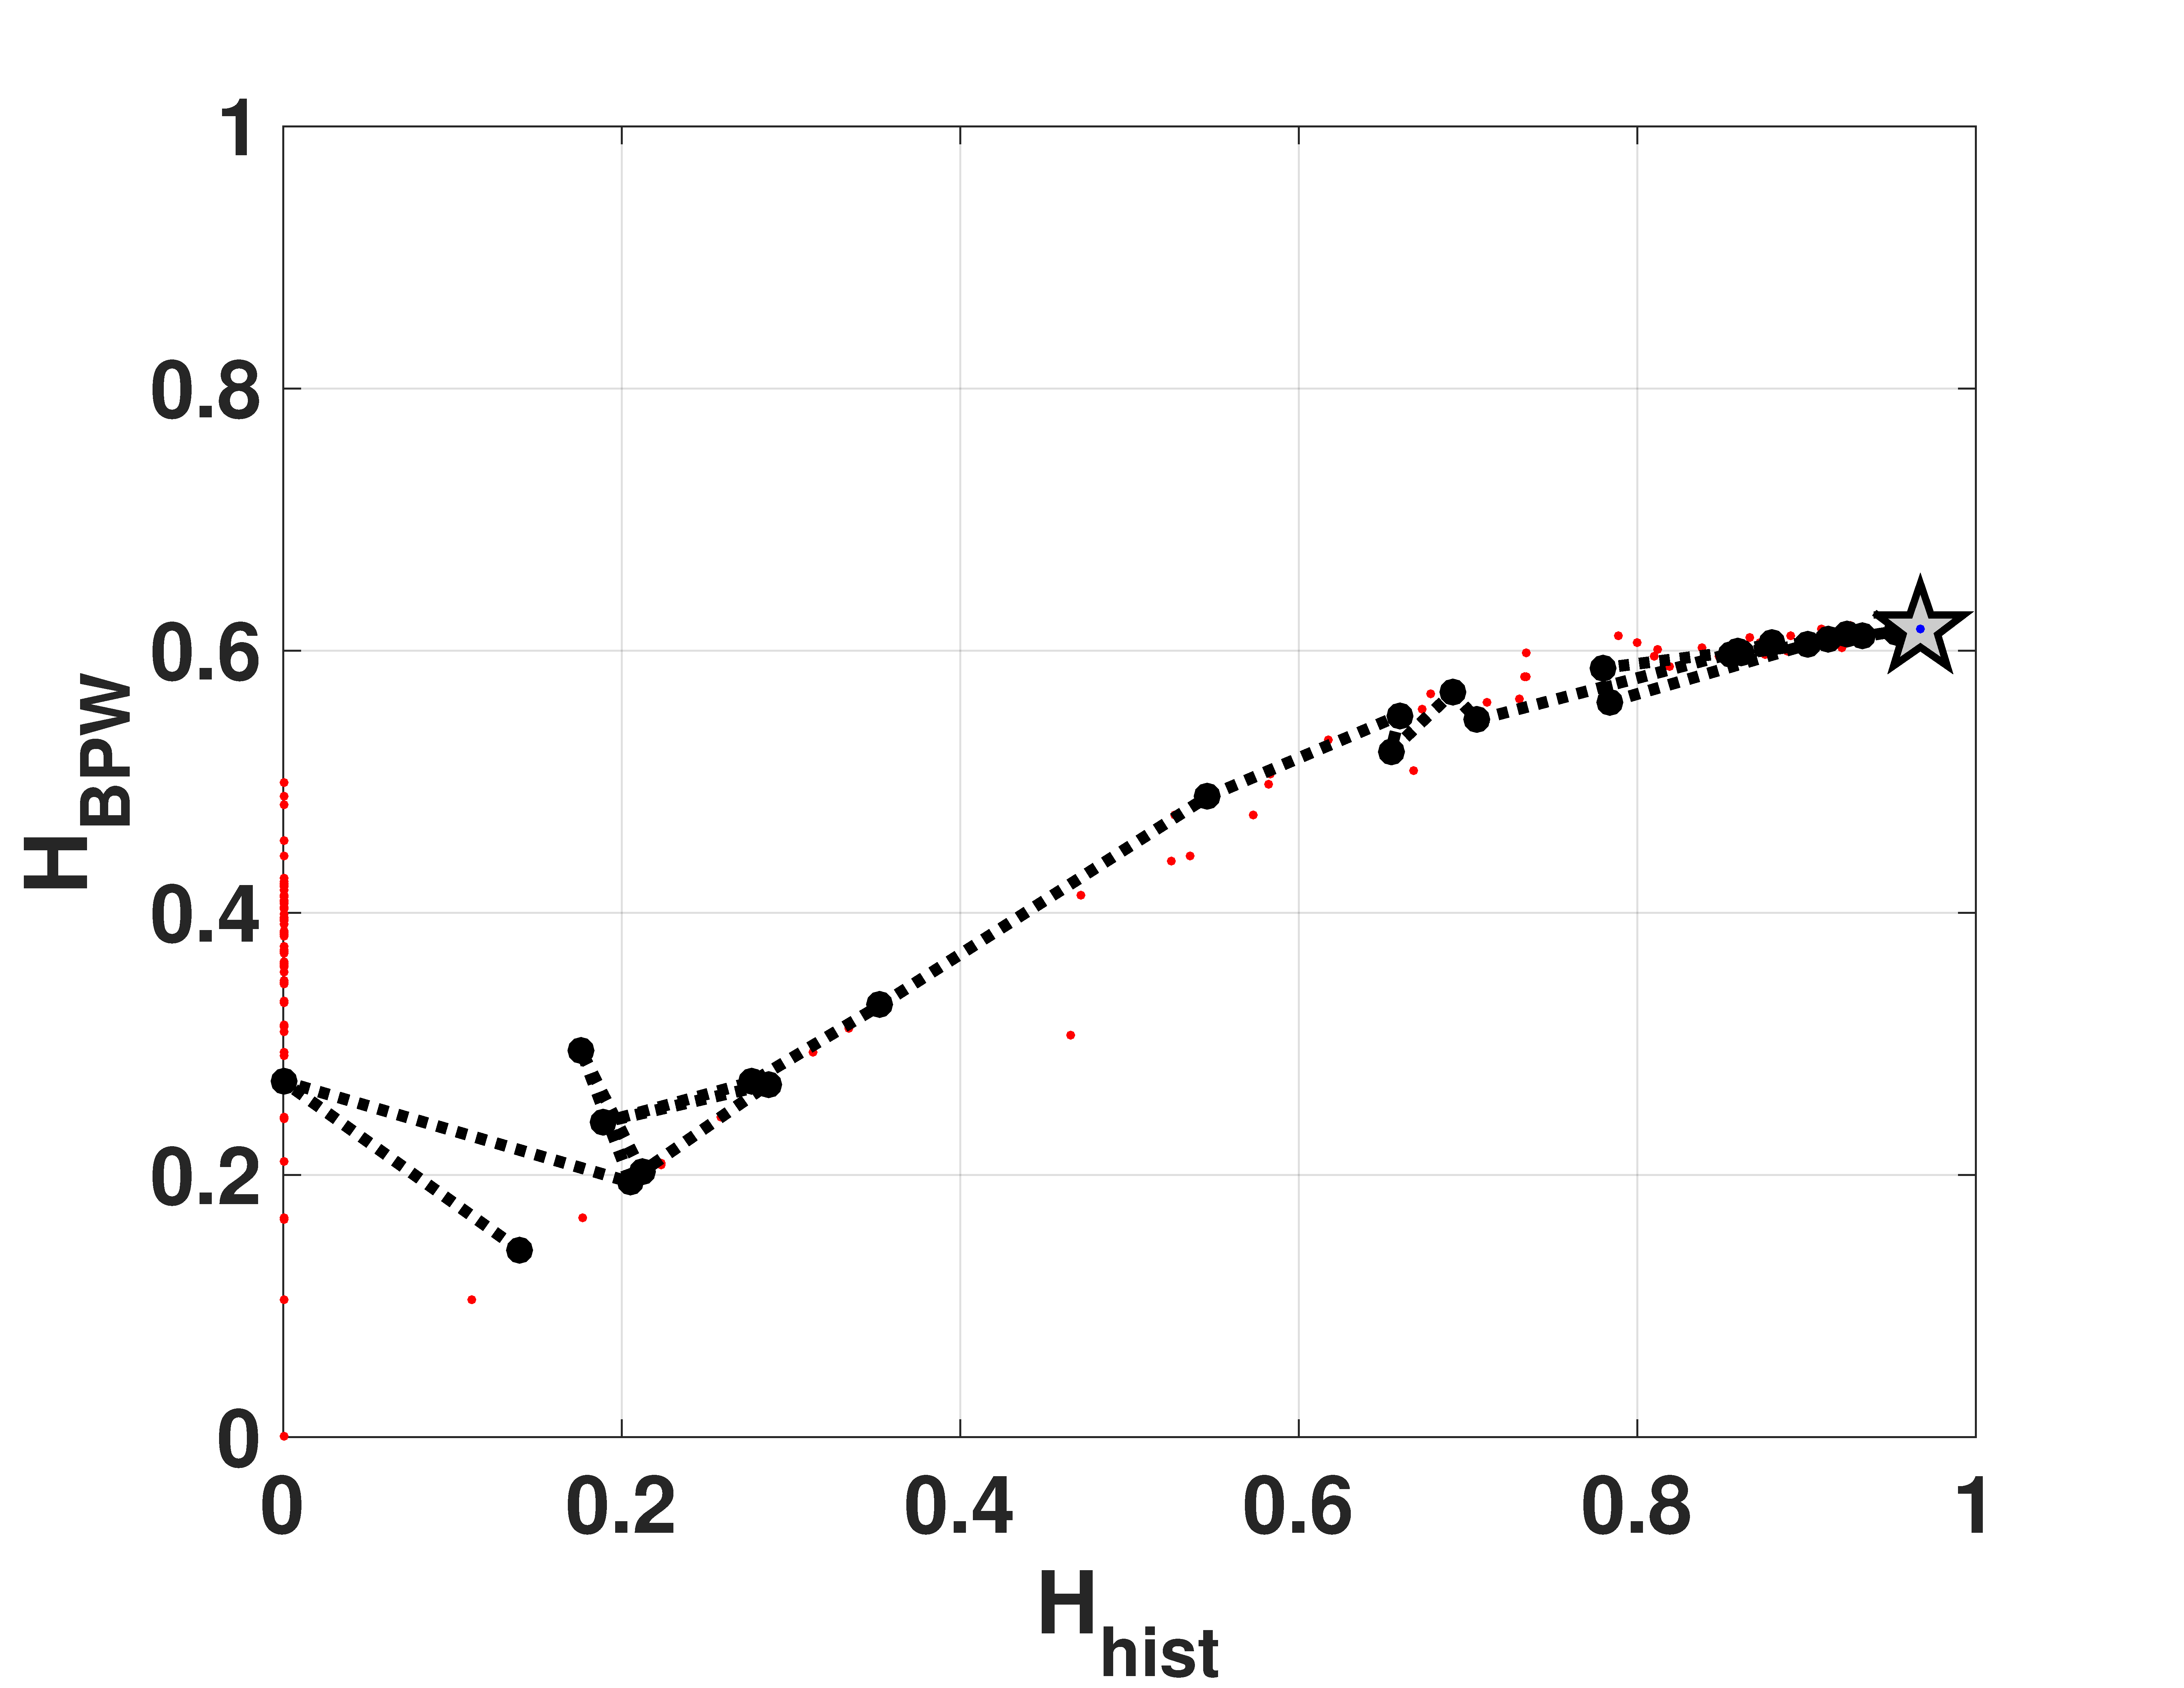
\includegraphics[width=\textwidth]{HbpwHval_Log}
		\caption{$H_{hist} \times H_{BPW}$}
		\label{fig:HbpwHval_Log}
	\end{subfigure}
	\caption{evolución de las propiedades estadísticas en el plano de doble entropía para el mapa LOG.}
	\label{fig:LOG_HH}
\end{figure}

En la Fig. \ref{fig:CbpHbp_Log} y \ref{fig:CbpwHbpw_Log}, mostramos los planos entropía - complejidad.
Las líneas grises punteadas son los márgenes superior e inferior, se espera que un sistema caótico permanezca cerca del margen superior.
Estos resultados caracterizan un comportamiento caótico, en el plano $H_{BP} \times C_{BP}$ podemos ver una baja entropía y alta complejidad.
%
\begin{figure}[htpb]
	\centering
	\begin{subfigure}[b]{0.49\textwidth}
		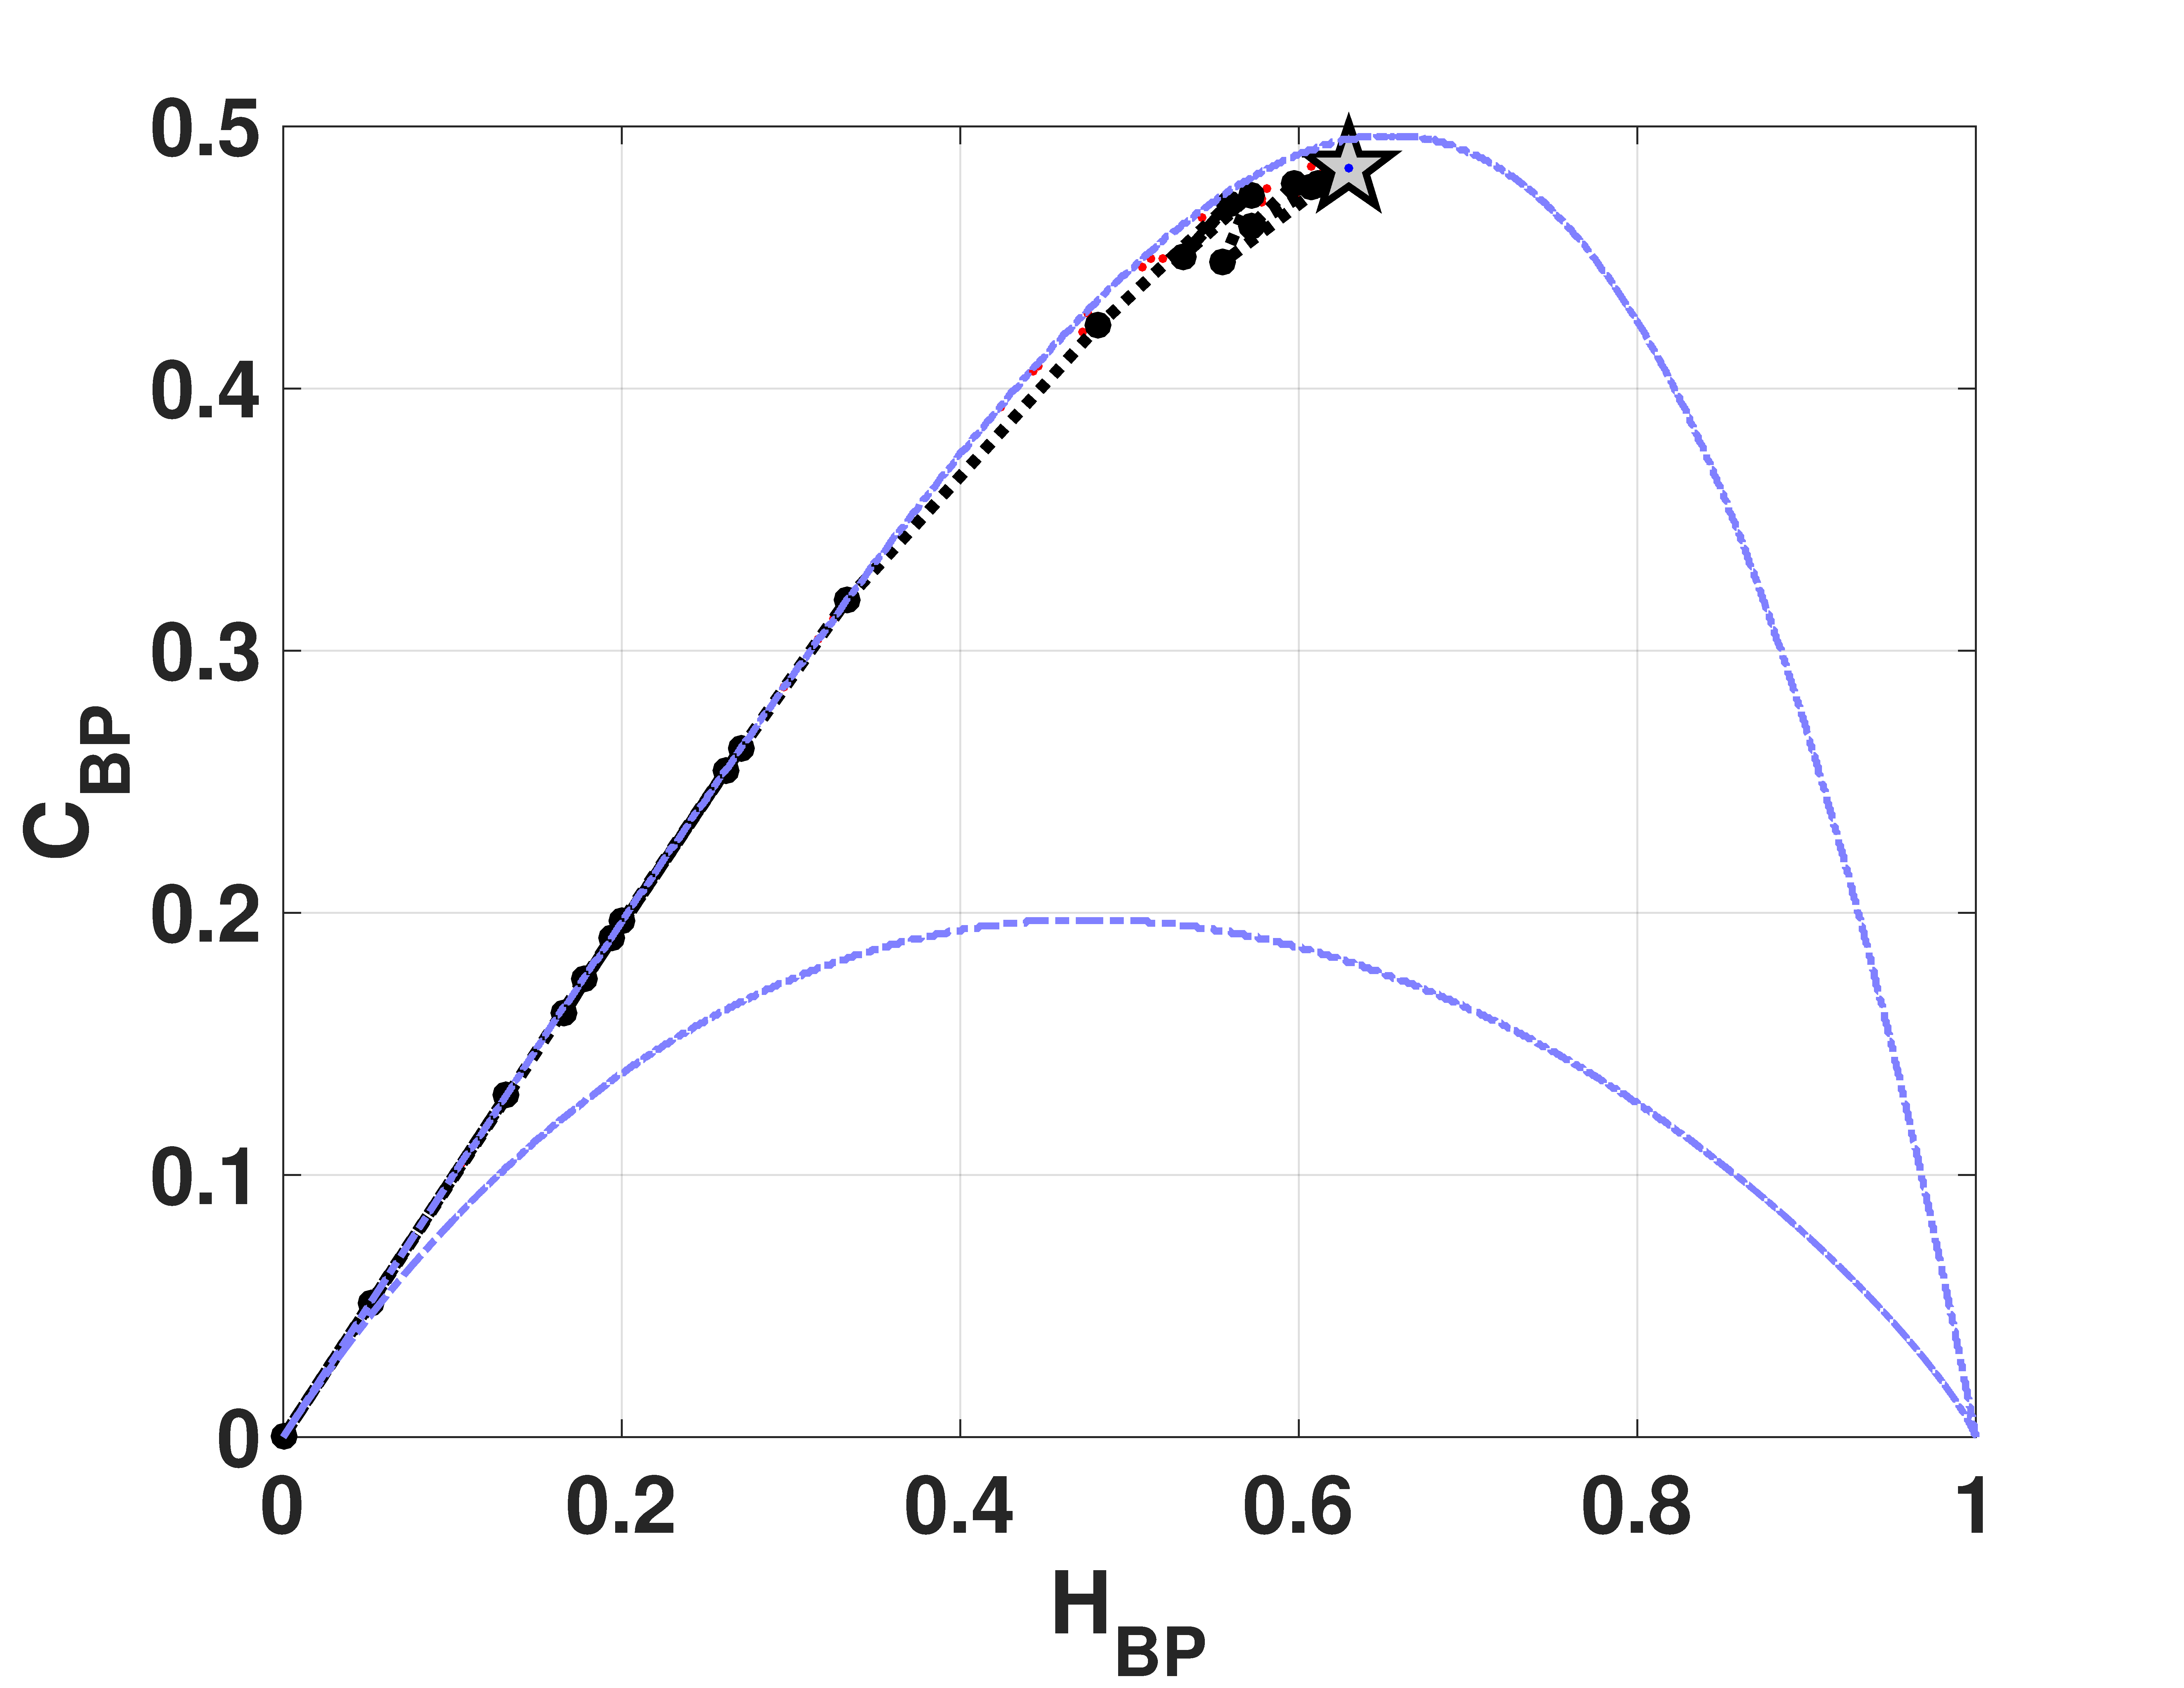
\includegraphics[width=\textwidth]{CbpHbp_Log}
		\caption{$H_{BP} \times C_{BP}$}
		\label{fig:CbpHbp_Log}
	\end{subfigure}
	\begin{subfigure}[b]{0.49\textwidth}
		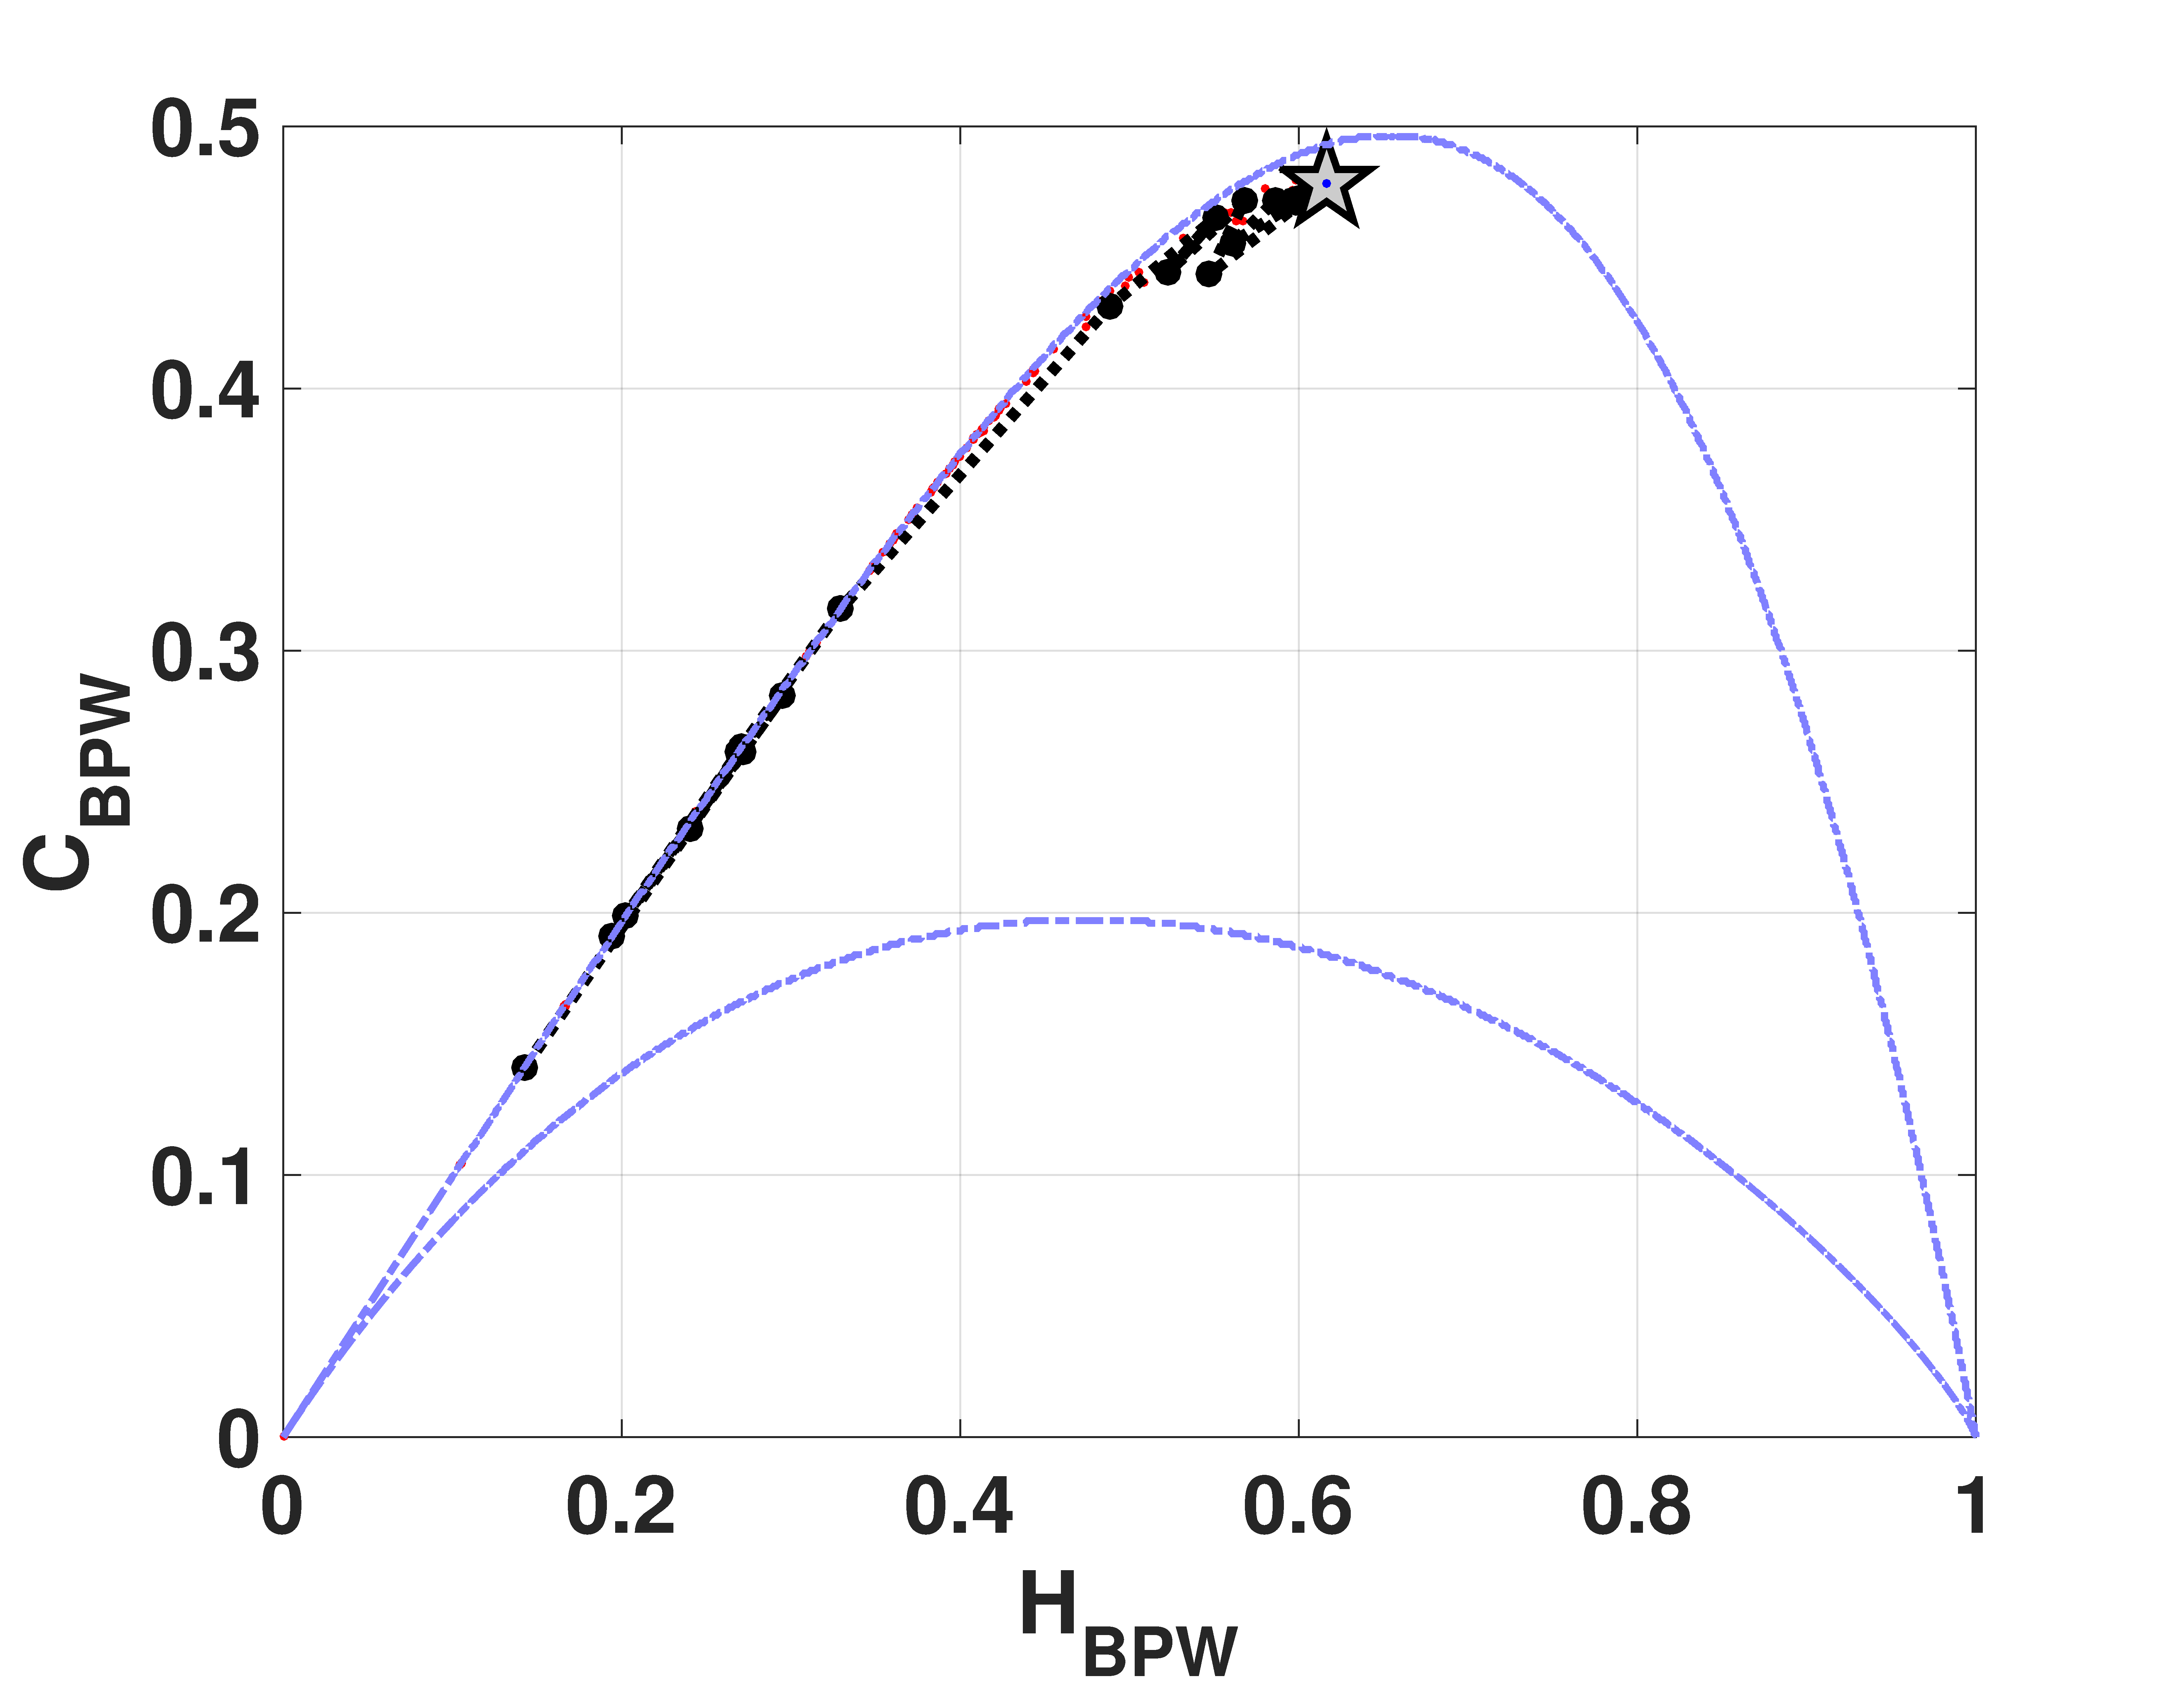
\includegraphics[width=\textwidth]{CbpwHbpw_Log}
		\caption{$H_{BPW} \times C_{BPW}$}
		\label{fig:CbpwHbpw_Log}
	\end{subfigure}
	\caption{Evolution of statistical properties in causal entropy-complexity plane for LOG map}
	\label{fig:LOG_HC}
\end{figure}
